\documentclass{article}
% --- Korean translation support (xelatex + kotex) ---
\usepackage{kotex}
\usepackage{fontspec}
\setmainfont{NanumMyeongjo}[AutoFakeSlant=0.167]
\setsansfont{NanumGothic}[AutoFakeSlant=0.167]
\setmainhangulfont{NanumMyeongjo}[AutoFakeSlant=0.167]
\setsanshangulfont{NanumGothic}[AutoFakeSlant=0.167]
\setmonohangulfont{NanumGothicCoding}[AutoFakeSlant=0.167]
\setmonofont{NanumGothicCoding}[AutoFakeSlant=0.167]
\linespread{1.22}\selectfont
\renewcommand{\figurename}{그림}
\renewcommand{\tablename}{표}
\setlength{\parindent}{1.2em}
% --- end Korean support ---
\usepackage{leaplab}

\usepackage[table,x11names]{xcolor}
\usepackage{relsize}        %

\usepackage[utf8]{inputenc} %
\usepackage[T1]{fontenc}    %
\usepackage{url}            %
\usepackage{booktabs}       %
\usepackage{amsfonts}       %
\usepackage{nicefrac}       %
\usepackage{microtype}      %
\usepackage{tabularx}   %
\usepackage{enumitem}

\usepackage[utf8]{inputenc} %
\usepackage[T1]{fontenc}    %
\usepackage{url}            %
\usepackage{booktabs}       %
\usepackage{amsfonts}       %
\usepackage{nicefrac}       %
\usepackage{microtype}      %
\definecolor{citecolor}{HTML}{0071bc}
\definecolor{shadecolor}{HTML}{EFEFEF}
\definecolor{linkcolor}{HTML}{9A4D92}
\usepackage{xurl}
\usepackage[colorlinks, linkcolor=linkcolor, anchorcolor=blue, citecolor=citecolor, pagebackref=True]{hyperref}


\usepackage{amsmath}
\usepackage{amssymb}
\usepackage{mathtools}
\usepackage{amsthm}
\usepackage{bm}
\usepackage{dsfont}
\usepackage{microtype}
\usepackage{graphicx}
\usepackage{booktabs} %
\usepackage{caption}
\usepackage{wrapfig}
\usepackage{float}
\usepackage{stfloats}

\usepackage{titletoc} %

\usepackage{subcaption}
\usepackage[export]{adjustbox}
\usepackage{footnote}
\usepackage{tablefootnote}
\usepackage{threeparttable}
\usepackage[capitalize,noabbrev]{cleveref}

% tabularray is unused in this source and unavailable in local TeX Live 2021
% \usepackage{tabularray}
% \UseTblrLibrary{booktabs}
\usepackage{multirow}
\usepackage{multicol}
\usepackage{xspace}
\usepackage{mathrsfs}
\usepackage{pifont}
\usepackage{makecell}
\usepackage{CJK}

\usepackage{marvosym} %
\usepackage[most]{tcolorbox}

\newcommand{\wzk}[1]{\begin{CJK}{UTF8}{gbsn}\textcolor{blue}{[wzk: #1]}\end{CJK}}
\newcommand{\YY}[1]{\begin{CJK}{UTF8}{gbsn}\textcolor{blue}{[YY: #1]}\end{CJK}}

\newcommand{\etal}{\textit{et al}.~}
\newcommand{\ie}{\textit{i}.\textit{e}.}
\newcommand{\ieno}{\textit{i}.\textit{e}.}
\newcommand{\eg}{\textit{e}.\textit{g}.}
\newcommand{\egno}{\textit{e}.\textit{g}.} %
\newcommand{\etc}{\textit{etc}.}
\newcommand{\etcno}{\textit{etc}} %
\renewcommand{\parallel}{\mathrel{/\mskip-4mu/}}\newcommand\blfootnote[1]{%
\begingroup
\renewcommand\thefootnote{}\footnote{#1}%
  \addtocounter{footnote}{-1}%
  \endgroup
}
\newcommand{\tablestyle}[2]{\setlength{\tabcolsep}{#1}\renewcommand{\arraystretch}{#2}\centering\footnotesize}
\newlength\savewidth\newcommand\shline{\noalign{\global\savewidth\arrayrulewidth
\global\arrayrulewidth 1pt}\hline\noalign{\global\arrayrulewidth\savewidth}}
\newcommand{\cmark}{\ding{51}}
\newcommand{\xmark}{\ding{55}}
\newcommand{\mask}{\texttt{[MASK]}\xspace}

\definecolor{lightblue}{RGB}{235, 242, 250} 
\definecolor{lightorange}{RGB}{255, 245, 235}
\newcommand{\gc}[1]{\textcolor{lightgray}{#1}}
\renewcommand{\paragraph}[1]{\noindent\textbf{#1}}


\definecolor{paleviolet}{HTML}{E1EEFC}
\definecolor{lightgrey}{RGB}{247, 247, 247}
\definecolor{darkgrey}{rgb}{0.5, 0.5, 0.5}
\definecolor{darkgreen}{rgb}{0, 0.5, 0}
\newenvironment{leapabstract}{
  \begin{tcolorbox}[
    colback=lightgrey,
    colframe=white,
    boxrule=0pt,
    arc=10pt,
    left=16pt,
    right=16pt,
    top=12pt,
    bottom=12pt,
    width=\textwidth,
    enlarge left by=0mm,
    before skip=10pt,
    after skip=10pt
  ]
}{
  \end{tcolorbox}
}


\begin{document}


\makeatletter
\def\icmldate#1{\gdef\@icmldate{#1}}
\icmldate{\today}
\makeatother

\makeatletter
\fancypagestyle{fancytitlepage}{
  \fancyhead{}  %
  \lhead{
\includegraphics[height=1.5cm]{figures/logos/leap.png}}
  \rhead{\it \@icmldate}
  \cfoot{}
}
\makeatother

\icmltitlerunning{The Flexibility Trap}

\icmltitle{유연성의 함정: Diffusion Language Models에서 arbitrary order의 가치 재고}

\vskip -.05in

\begin{icmlauthorlist}
\mbox{Zanlin Ni$^{\,1\,}$},
\mbox{Shenzhi Wang$^{\,1}$},
\mbox{Yang Yue$^{\,1}$},
\mbox{Tianyu Yu$^{\,2}$},
\mbox{Weilin Zhao$^{\,2}$},
\mbox{Yeguo Hua$^{\,3}$},
\mbox{Tianyi Chen$^{\,3}$},
\mbox{Jun Song$^{\,4}$},
\mbox{Cheng Yu$^{\,4}$},
\mbox{Bo Zheng$^{\,4}$},
\mbox{Gao Huang$^{\,1,5\,\textrm{\Letter}}$}
\end{icmlauthorlist}

$^{1\,}$ LeapLab, Tsinghua University  \quad $^{2\,}$ NLPLab, Tsinghua University \\
\quad $^{3\,}$ Tsinghua University \quad $^{4\,}$ Alibaba Group \quad $^{5\,}$ BNRist, Tsinghua University

{
\smaller
\texttt{nzl22@mails.tsinghua.edu.cn, gaohuang@tsinghua.edu.cn}
}

\icmlcorrespondingauthor{gaohuang@tsinghua.edu.cn}


\vskip -1in


\begin{leapabstract}
    Diffusion Large Language Models (dLLMs)는 전통적인 LLM의 엄격한 left-to-right 제약을 깨고, token을 arbitrary order로 생성할 수 있게 한다.
직관적으로 이러한 유연성은 고정된 autoregressive trajectory를 엄격히 포함하는 solution space를 의미하며, 이론적으로 더 뛰어난 reasoning 잠재력을 열어 준다.
하지만 이 논문에서 우리는 일반 reasoning task(\eg, 수학과 코딩)의 경우 arbitrary order generation이 실제로는 dLLM의 reasoning 잠재력을 제한할 수 있음을 발견한다.
우리는 dLLM이 exploration에 중요한 high-uncertainty token을 우회하기 위해 이러한 순서 유연성을 활용하는 경향이 있으며, 이는 solution coverage의 조기 붕괴로 이어질 수 있음을 관찰한다.
이 관찰은 dLLM을 위한 RL 접근법을 재고하도록 동기를 부여한다. 기존 접근법에서는 combinatorial trajectory와 다루기 어려운 likelihood를 처리하는 등 상당한 복잡성이 종종 이러한 유연성을 보존하는 데 투입된다.
우리는 arbitrary order를 단순히 포기하고 대신 표준 Group Relative Policy Optimization (GRPO)을 적용하는 것만으로 효과적인 reasoning을 이끌어낼 수 있음을 보인다.
우리의 접근법인 \textbf{JustGRPO}는 미니멀하지만 놀라울 정도로 효과적이며(\eg, GSM8K에서 89.1\% 정확도), dLLM의 parallel decoding 능력은 완전히 유지한다.
\begin{center}
    프로젝트 페이지: \url{https://nzl-thu.github.io/the-flexibility-trap}
\end{center}

\end{leapabstract}


\section{서론}
\label{sec:intro}

최근 연구에서는 Diffusion Large Language Models (dLLMs)~\cite{nie2025large,ye2025dream,zhu2025llada,zhao2025d1,labs2025mercury}가 급증하고 있다. dLLM은 sequence generation을 이산 denoising 과정으로 취급함으로써 지배적인 autoregressive (AR) 패러다임~\cite{brown2020language,achiam2023gpt}에 도전한다.
dLLM의 매력의 핵심은 이론적 유연성에 있으며, 이는 AR model의 엄격한 left-to-right causal chain에 비해 두 가지 뚜렷한 장점을 제공한다: 효율적인 parallel decoding과 arbitrary-order generation 능력이다.

parallel decoding의 효율성 이득은 이미 잘 확립되어 있지만~\cite{fastdllm,labs2025mercury,geminidiffusion,song2025seed,wu2025fast}, arbitrary-order generation의 함의는 상대적으로 덜 탐구되었다.
이론적으로 제약 없는 생성 순서는 고정된 autoregressive trajectory의 상위집합을 이루며, 더 발전된 문제 해결 능력을 열어 줄 잠재력을 가진다.
한편 일부 연구~\cite{ye2024beyond,kim2025train}는 스도쿠와 zebra puzzle 같은 특정 과제에서 non-sequential generation의 우수성을 입증했다.
이러한 성공과 이론적 가능성에 힘입어, 커뮤니티는 수학과 코딩 같은 \emph{일반 reasoning task}에서 유사한 고급 능력을 이끌어내기 위해 Reinforcement Learning (RL)을 점점 더 많이 채택해 왔다\footnote{
    우리는 이러한 도메인이 폭넓은 실용적 유용성과 reasoning model의 핵심 지능을 벤치마킹하는 중심적 역할을 지닌다는 점에서 \emph{일반 reasoning}의 주요 대표로 초점을 맞춘다.
    }~\cite{zhao2025d1,wang2025spg,gong2025diffucoder,rojas2025improving,ou2025principled}.

이 연구에서 우리는 반직관적인 관찰을 제시한다: 이러한 일반 reasoning task에서는 arbitrary-order generation이 RL로 이끌어낼 수 있는 reasoning 잠재력을 확장하기보다 오히려 좁힐 수 있다.
이를 엄밀히 평가하기 위해 우리는 solution space의 coverage를 측정하는 Pass@$k$~\cite{chen2021evaluating}를 사용한다.
최근 연구들은 RL이 주로 base model의 분포를 날카롭게 만드는 역할을 한다고 시사한다. 따라서 base model의 Pass@$k$ 성능은 RL 학습 후 모델이 달성 가능한 reasoning 한계에 대한 효과적인 proxy가 된다~\cite{yue2025does,liu2025prorl}.
이 지표 아래에서 우리는 LLaDA-Instruct~\cite{nie2025large}를 사용하여 arbitrary-order generation의 reasoning 잠재력을 표준 AR decoding과 비교한다.
Figure~\ref{fig:teaser}(왼쪽)에 보이듯, dLLM을 표준 AR order로 제한하면 유연한 counterpart보다 \emph{더 높은} Pass@$k$, 그리고 결과적으로 더 높은 reasoning boundary를 산출하는 경향이 있다.

\begin{figure}[t]\centering
    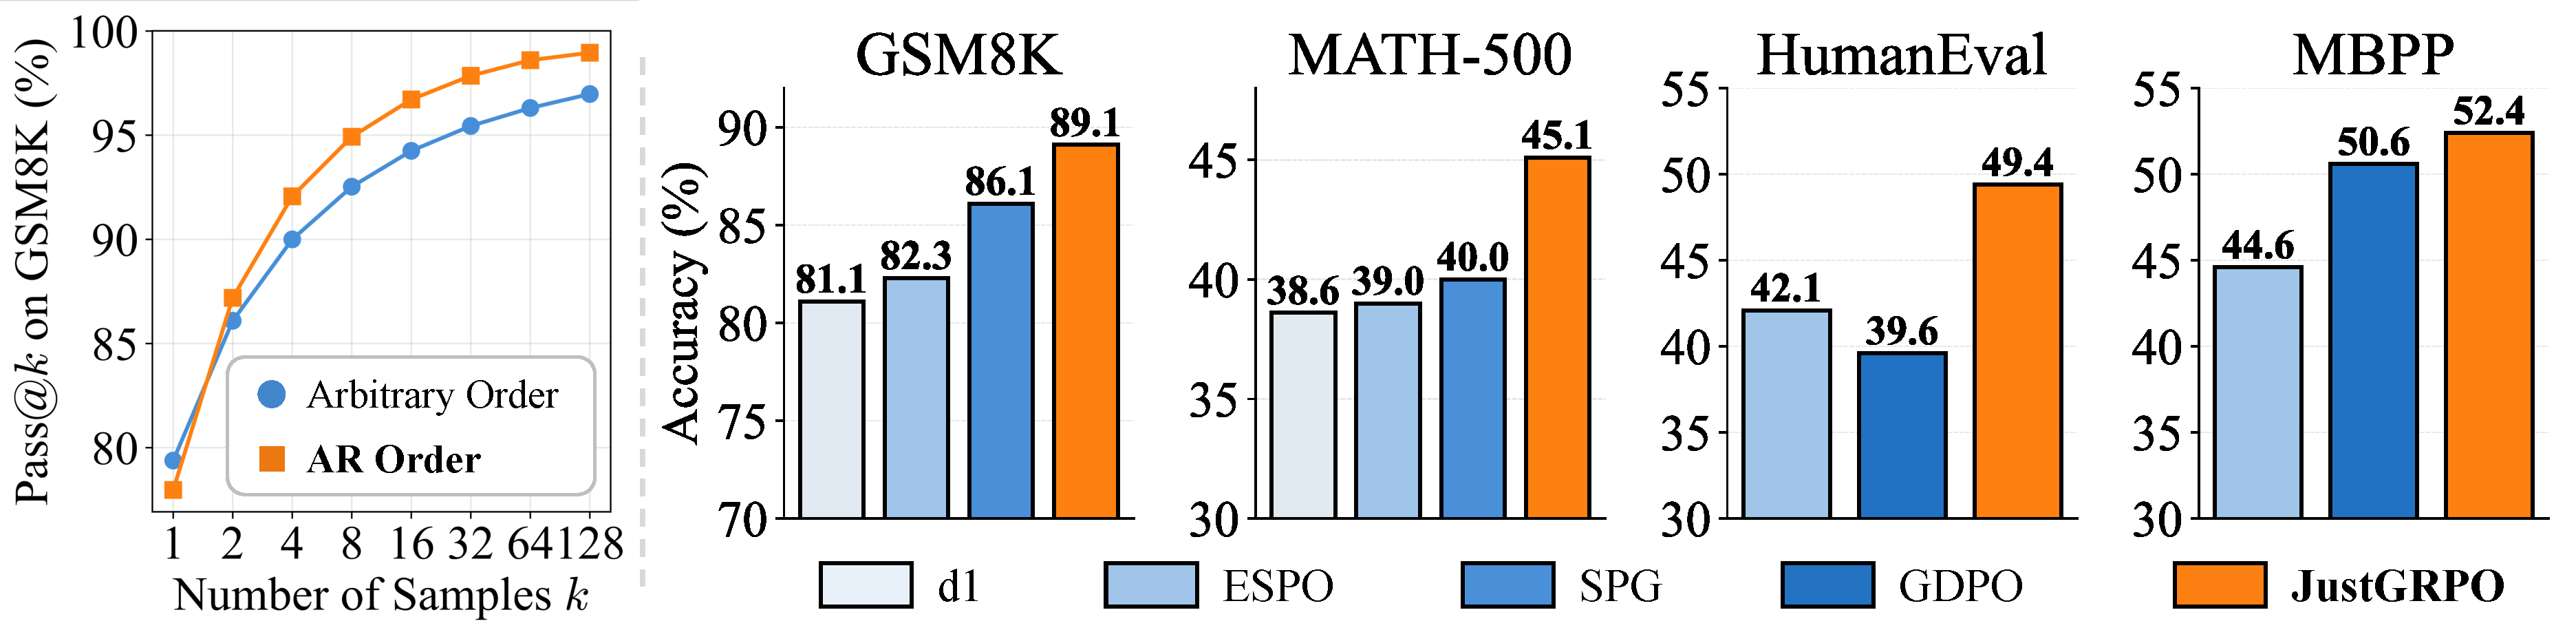
\includegraphics[width=\linewidth]{figures/teaser.pdf}
    \caption{
    \textbf{더 적은 유연성이 더 나은 reasoning 잠재력을 연다.}
    \emph{왼쪽}: dLLM을 표준 Autoregressive (AR) order로 제한하면 reasoning solution space가 확장되는 반직관적인 현상을 관찰한다.
    \emph{오른쪽}: 이에 동기를 받아 우리는 ``\textbf{JustGRPO}''를 제안한다. arbitrary-order adaptation을 포기하고 단지 GRPO를 채택함으로써, dLLM의 reasoning capability를 더 효과적으로 이끌어낸다. 결과는 생성 길이 256에서 LLaDA-Instruct~\cite{nie2025large}에 대해 보고했다. Baseline 결과는 해당 논문에서 인용했다. 또한 Table~\ref{tab:controlled_comparison}에는 맞춘 설정에서 재현한 결과도 포함한다.
    \label{fig:teaser}
    }
\end{figure}



이 반직관적인 관찰은 서로 다른 순서가 uncertainty를 처리하는 방식과 밀접하게 관련된다.
\begin{wrapfigure}{r}{0.52\textwidth}
    \centering
    \vskip -0.12in
    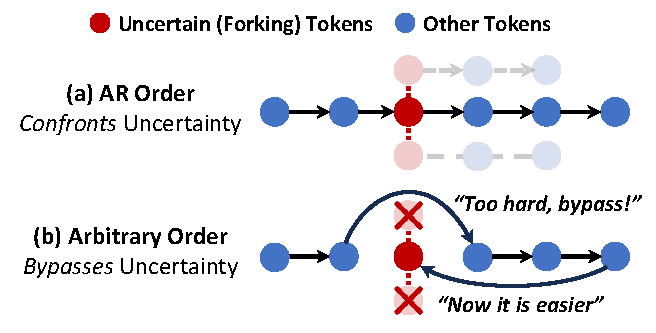
\includegraphics[width=\linewidth]{figures/illustrate.pdf}
    \vskip -0.10in
    \caption{
        \textbf{uncertainty에 맞서기 \emph{vs.} 우회하기.}
        (a) \textbf{AR order}는 uncertain token에서 결정을 강제함으로써 reasoning space를 보존한다.
        (b) \textbf{Arbitrary order}는 uncertainty를 우회하고 더 쉬운 token을 먼저 해결한다.
        미래 context가 확립되면, 원래의 branching 가능성은 사실상 pruning된다.
        \label{fig:illustrate}
    }
    \vskip -0.12in
\end{wrapfigure}
reasoning은 본질적으로 균일하지 않다. reasoning은 드문드문 나타나는 ``forking token''에 달려 있으며, 이는 보통 ``Therefore''나 ``Since'' 같은 연결어로서 단순히 문장을 이어 가는 것이 아니라 논리적 trajectory를 서로 다른 branch로 이끈다~\cite{wang2025beyond,cheng2025reasoning,huang2025low}.
이러한 fork에서 reasoning path는 갈라지며, 자연스럽게 entropy의 국소적 spike로 나타난다~\cite{wang2025beyond}.
표준 AR decoding은 모델이 이 uncertainty에 \emph{맞서도록} 강제한다(Figure~\ref{fig:illustrate}a).
바로 이러한 fork에서 sampling함으로써 모델은 서로 다른 reasoning path를 탐색할 수 있고, 따라서 생성된 rationale의 다양성을 보존한다.
반면 arbitrary-order generation은 모델이 이러한 어려운 결정을 \emph{우회할} 수 있게 한다(Figure~\ref{fig:illustrate}b).
이 유연성은 일반적으로 low-uncertainty token을 우선하기 위해 활용되며~\cite{nie2025large}, 이는 그 token으로 이어지는 연결어를 결정하기 전에 더 쉬운 부분에서 reasoning path를 사실상 고정한다.
모델이 우회한 fork를 infill하기 위해 돌아올 때쯤에는, 이미 확립된 미래 context가 그 ambiguity를 조기에 해소해 버린다.
우리는 이 현상을 \emph{entropy degradation}이라 부른다: fork에 원래 내재했던 high entropy가 억제되는 것이다.
결과적으로 모델은 더 이상 branching point를 탐색하는 것이 아니라, 사전에 결정된 gap을 잇도록 연결어를 맞추고 있을 뿐이다.





위 관찰은 이러한 일반 reasoning task에서 dLLM을 위한 RL을 재고하도록 동기를 부여한다.
현재 방법들은 arbitrary-order 유연성을 보존하는 것이 필수적이라는 가정 아래 작동한다. 이러한 고수에는 큰 비용이 따른다. 알고리즘은 denoising trajectory의 combinatorial explosion~\cite{zhao2025d1,yang2025mmada,gong2025diffucoder}과 다루기 어려운 marginal likelihood~\cite{ou2025principled,wang2025spg}에 맞서야 하며, 부정확한 approximation~\cite{wang2025spg,ou2025principled,rojas2025improving}에 의존할 수밖에 없다.
하지만 arbitrary order가 target task의 잠재력을 이끌어내는 데 필수적이지 않거나 심지어 해롭다면, 이러한 복잡성은 불필요할 수 있다.

이를 위해 우리는 \textbf{JustGRPO}를 통해 단순성으로 돌아갈 것을 제안한다.
우리는 일반 reasoning task의 reasoning 잠재력을 이끌어내는 데 복잡한 diffusion-specific RL adaptation이 반드시 필요한 것은 아님을 보인다.
대신 RL 학습 중 dLLM을 단순히 AR policy로 취급함으로써 효과적으로 달성할 수 있다. 이를 통해 표준 GRPO~\cite{shao2024deepseekmath}를 수정 없이 적용하여, 그렇지 않았다면 다루기 어려운 optimization을 잘 정의된 과제로 바꾼다.
중요하게도, 이 AR formulation은 더 나은 exploration을 위해 RL 학습 중에만 ``scaffold'' 역할을 한다.
dLLM의 고유 architecture는 그대로 유지된다. \eg, causal masking을 부과하지 않으므로 bidirectional attention과 discrete diffusion formulation이 보존된다.
그 결과 \textit{reasoning ability의 elicitation}(sequential exploration의 이점을 얻음)과 \textit{inference execution}(dLLM의 parallel decoding 이점을 얻음)이 분리된다. 


단순함에도 불구하고 JustGRPO는 놀라울 정도로 효과적이다.
이는 강한 결과(\eg, GSM8K에서 89.1\% 정확도, MATH-500에서 45.1\%)를 달성하며, 복잡한 diffusion-specific RL adaptation에 의존하는 방법들과 비교해도 우수하다(Table~\ref{tab:main_results}).
더 중요하게는 Figure~\ref{fig:eb_sampler_comparison}에 보이듯, AR-trained model은 parallel decoding과 완전히 호환된 상태로 남아 있어, AR exploration을 통해 획득한 reasoning capability가 dLLM의 대표적인 inference efficiency를 희생할 필요가 없음을 시사한다.


\section{배경}
\label{sec:prelim}
\subsection{Diffusion Large Language Models}

Diffusion Large Language Models (dLLMs), 특히 Masked Diffusion Models (MDMs)는 완전히 mask된 token에서 초기화된 masked state $x_t$를 반복적으로 denoise함으로써 sequence를 생성한다. 이 과정은 masking ratio를 나타내는 연속 시간 변수 $t \in [0,1]$로 index된다.
깨끗한 sequence $x_0$가 주어지면, forward process는 각 token을 확률 $t$로 독립적으로 mask한다:
\begin{equation}
q(x_{t,k} \mid x_{0,k}) =
\begin{cases}
\mask, & \text{확률 } t, \\
x_{0,k}, & \text{확률 } 1 - t,
\end{cases}
\end{equation}
여기서 $k$는 token index이다.
Neural network $p_\theta(x_0 \mid x_t)$는 masked position에서 원래 token distribution을 추정한다. Inference 중에는 $x_1$(모두 \mask)에서 generation을 시작하고 confidence score 같은 heuristic에 기반해 token subset의 mask를 반복적으로 제거하며, 완료될 때까지 $x_t \rightarrow x_{t-\Delta t}$를 업데이트한다. 특수한 경우로서 dLLM은 항상 가장 왼쪽 token의 mask를 제거함으로써 autoregressive하게 generation을 수행할 수도 있다.
모델은 Negative Evidence Lower Bound를 최소화하여 학습되며, 이는 masked token에 대한 weighted cross entropy loss로 환원된다:
\begin{equation}
\mathcal{L}_{\mathrm{MDM}}(\theta)
= -\mathbb{E}_{t \sim \mathcal{U}[0,1],\, x_t \sim q(x_t \mid x_0)}
\left[
\frac{1}{t}
\sum_{k=1}^{L}
\mathbf{1}[x_{t,k} = \mask]\,
\log p_\theta(x_{0,k} \mid x_t)
\right].
\end{equation}

\subsection{Group Relative Policy Optimization}
\label{sec:prelim_grpo}

Group Relative Policy Optimization (GRPO)은 group level reward normalization을 사용하여 value function estimation을 피하는 reinforcement learning 알고리즘이다. 이는 일반적으로 autoregressive policy $\pi_\theta(o_k \mid o_{<k}, q)$에 적용된다.
각 query $q$에 대해 GRPO는 old policy $\pi_{\theta_{\text{old}}}$로부터 $G$개의 output group $\{o_1, \dots, o_G\}$를 sample한다. Advantage $\hat{A}_{i,k}$는 reward $r(o_i)$를 group statistics에 대해 standardize하여 계산된다: $\hat{A}_{i,k} = (r(o_i) - \mu_G) / \sigma_G$, 여기서 $\mu_G$와 $\sigma_G$는 group mean과 standard deviation이다.
GRPO objective는 KL regularization term이 포함된 clipped surrogate function을 최대화한다:
\begin{equation}
\mathcal{J}(\theta) = \mathbb{E}_{q \sim P(Q), \{o_i\}_{i=1}^G \sim \pi_{\theta_{\text{old}}}} \Bigg[ \frac{1}{G} \sum_{i=1}^G \frac{1}{|o_i|} \sum_{k=1}^{|o_i|} \Big( \min \big( \rho_{i,k} \hat{A}_{i,k}, \text{clip}(\rho_{i,k}, 1-\epsilon, 1+\epsilon) \hat{A}_{i,k} \big) - \beta \mathbb{D}_{\text{KL}} \Big) \Bigg]
\end{equation}
token level importance ratio는 $\rho_{i,k} = \frac{\pi_\theta(o_{i,k} \mid o_{i,<k}, q)}{\pi_{\theta_{\text{old}}}(o_{i,k} \mid o_{i,<k}, q)}$이다.

\subsection{Reasoning Potential의 Proxy로서 Pass@$k$}

dLLM의 reasoning capability boundary를 엄밀하게 정량화하기 위해 우리는 Pass@$k$ metric~\cite{chen2021evaluating,yue2025does}를 채택한다. 현재 reasoning capability를 향상시키는 지배적 패러다임인 Reinforcement Learning with Verifiable Rewards (RLVR)의 맥락에서, exploration은 개선의 전제조건이다. RL agent는 exploration phase에서 올바른 reasoning path를 sampling하여 positive reward signal을 얻을 수 있을 때에만 이를 강화할 수 있다.

따라서 Pass@$k$는 모델의 \textit{reasoning potential}에 대한 표준 measure로 널리 확립되어 왔다~\cite{yue2025does,liu2025prorl,zhang2025interplay}.
이는 $k$개의 독립 sample 안에서 적어도 하나의 correct solution이 생성될 확률을 측정하며, RL optimization이 접근 가능한 solution space의 upper bound를 효과적으로 나타낸다. 형식적으로, unbiased estimator formulation~\cite{chen2021evaluating,yue2025does}을 따르면, $n$개의 sample 중 $c$개가 correct일 때 Pass@$k$는 다음과 같이 계산된다:
\begin{equation}
\text{Pass@}k = \mathbb{E}\left[1 - \frac{\binom{n-c}{k}}{\binom{n}{k}}\right]
\end{equation}

높은 Pass@$k$는 올바른 reasoning trajectory가 모델의 sampling distribution 안에 있으며 따라서 RL optimization을 통해 학습 가능함을 나타낸다. 반대로, 막대한 sampling budget에도 불구하고 모델이 일관되게 solution을 산출하지 못한다면, 해당 문제가 모델의 intrinsic reasoning boundary 바깥에 있음을 시사한다. 이러한 시나리오에서 표준 RLVR 방법론은 positive exploration signal의 부재로 인해 근본적으로 제한된다~\cite{yue2025does}.

\section{Flexibility Trap}
\label{sec:rethink_value_of_AO}
이 절에서는 arbitrary-order generation의 유연성이 더 높은 reasoning 잠재력으로 이어지는지 실증적으로 검증한다.
우리는 두 가지 decoding 모드를 비교한다: 낮은 confidence의 remasking을 사용하는 표준 diffusion decoding을 따르는 \emph{Arbitrary Order}~\cite{nie2025large,zhao2025d1,fastdllm}와 arbitrary-order 유연성을 비활성화하고 생성을 엄격히 left-to-right decoding으로 제한하는 \emph{AR Order}이다. 
우리는 기존 diffusion LLM 연구에서 일반적으로 사용되는 실험 설정을 채택한다: 최대 256 tokens를 256 steps에 걸쳐 decoding하고, semi-autoregressive block size는 32로 둔다.
Sampling temperature는~\cite{yue2025does}와 같이 0.6으로 설정한다. Prompt template은~\cite{zhao2025d1}를 따른다.
대안적인 temperature와 sampling 구성에서의 결과는 Appendix~\ref{app:boundary_ablations}로 미룬다.

\subsection{Arbitrary Order는 Reasoning 잠재력을 제한할 수 있다}
\paragraph{Pass@$k$ analysis.}
먼저 네 가지 reasoning benchmarks인 GSM8K, MATH-500, HumanEval, MBPP에서 세 가지 대표적인 dLLMs: LLaDA-Instruct~\cite{nie2025large}, Dream-Instruct~\cite{ye2025dream}, LLaDA 1.5~\cite{zhu2025llada}에 대해 Pass@$k$ metric을 사용해 reasoning 잠재력을 평가한다.
Figure~\ref{fig:passk_comparison}에 보이듯, arbitrary order는 $k=1$에서 종종 경쟁력 있고 많은 경우 더 나은 성능을 달성하지만, AR mode와 비교하면 scaling curve가 눈에 띄게 더 평평하다. $k$가 증가함에 따라 AR mode는 더 많은 정답 solution을 찾아내는 더 강한 능력을 보인다. 



\begin{figure}[t]\centering
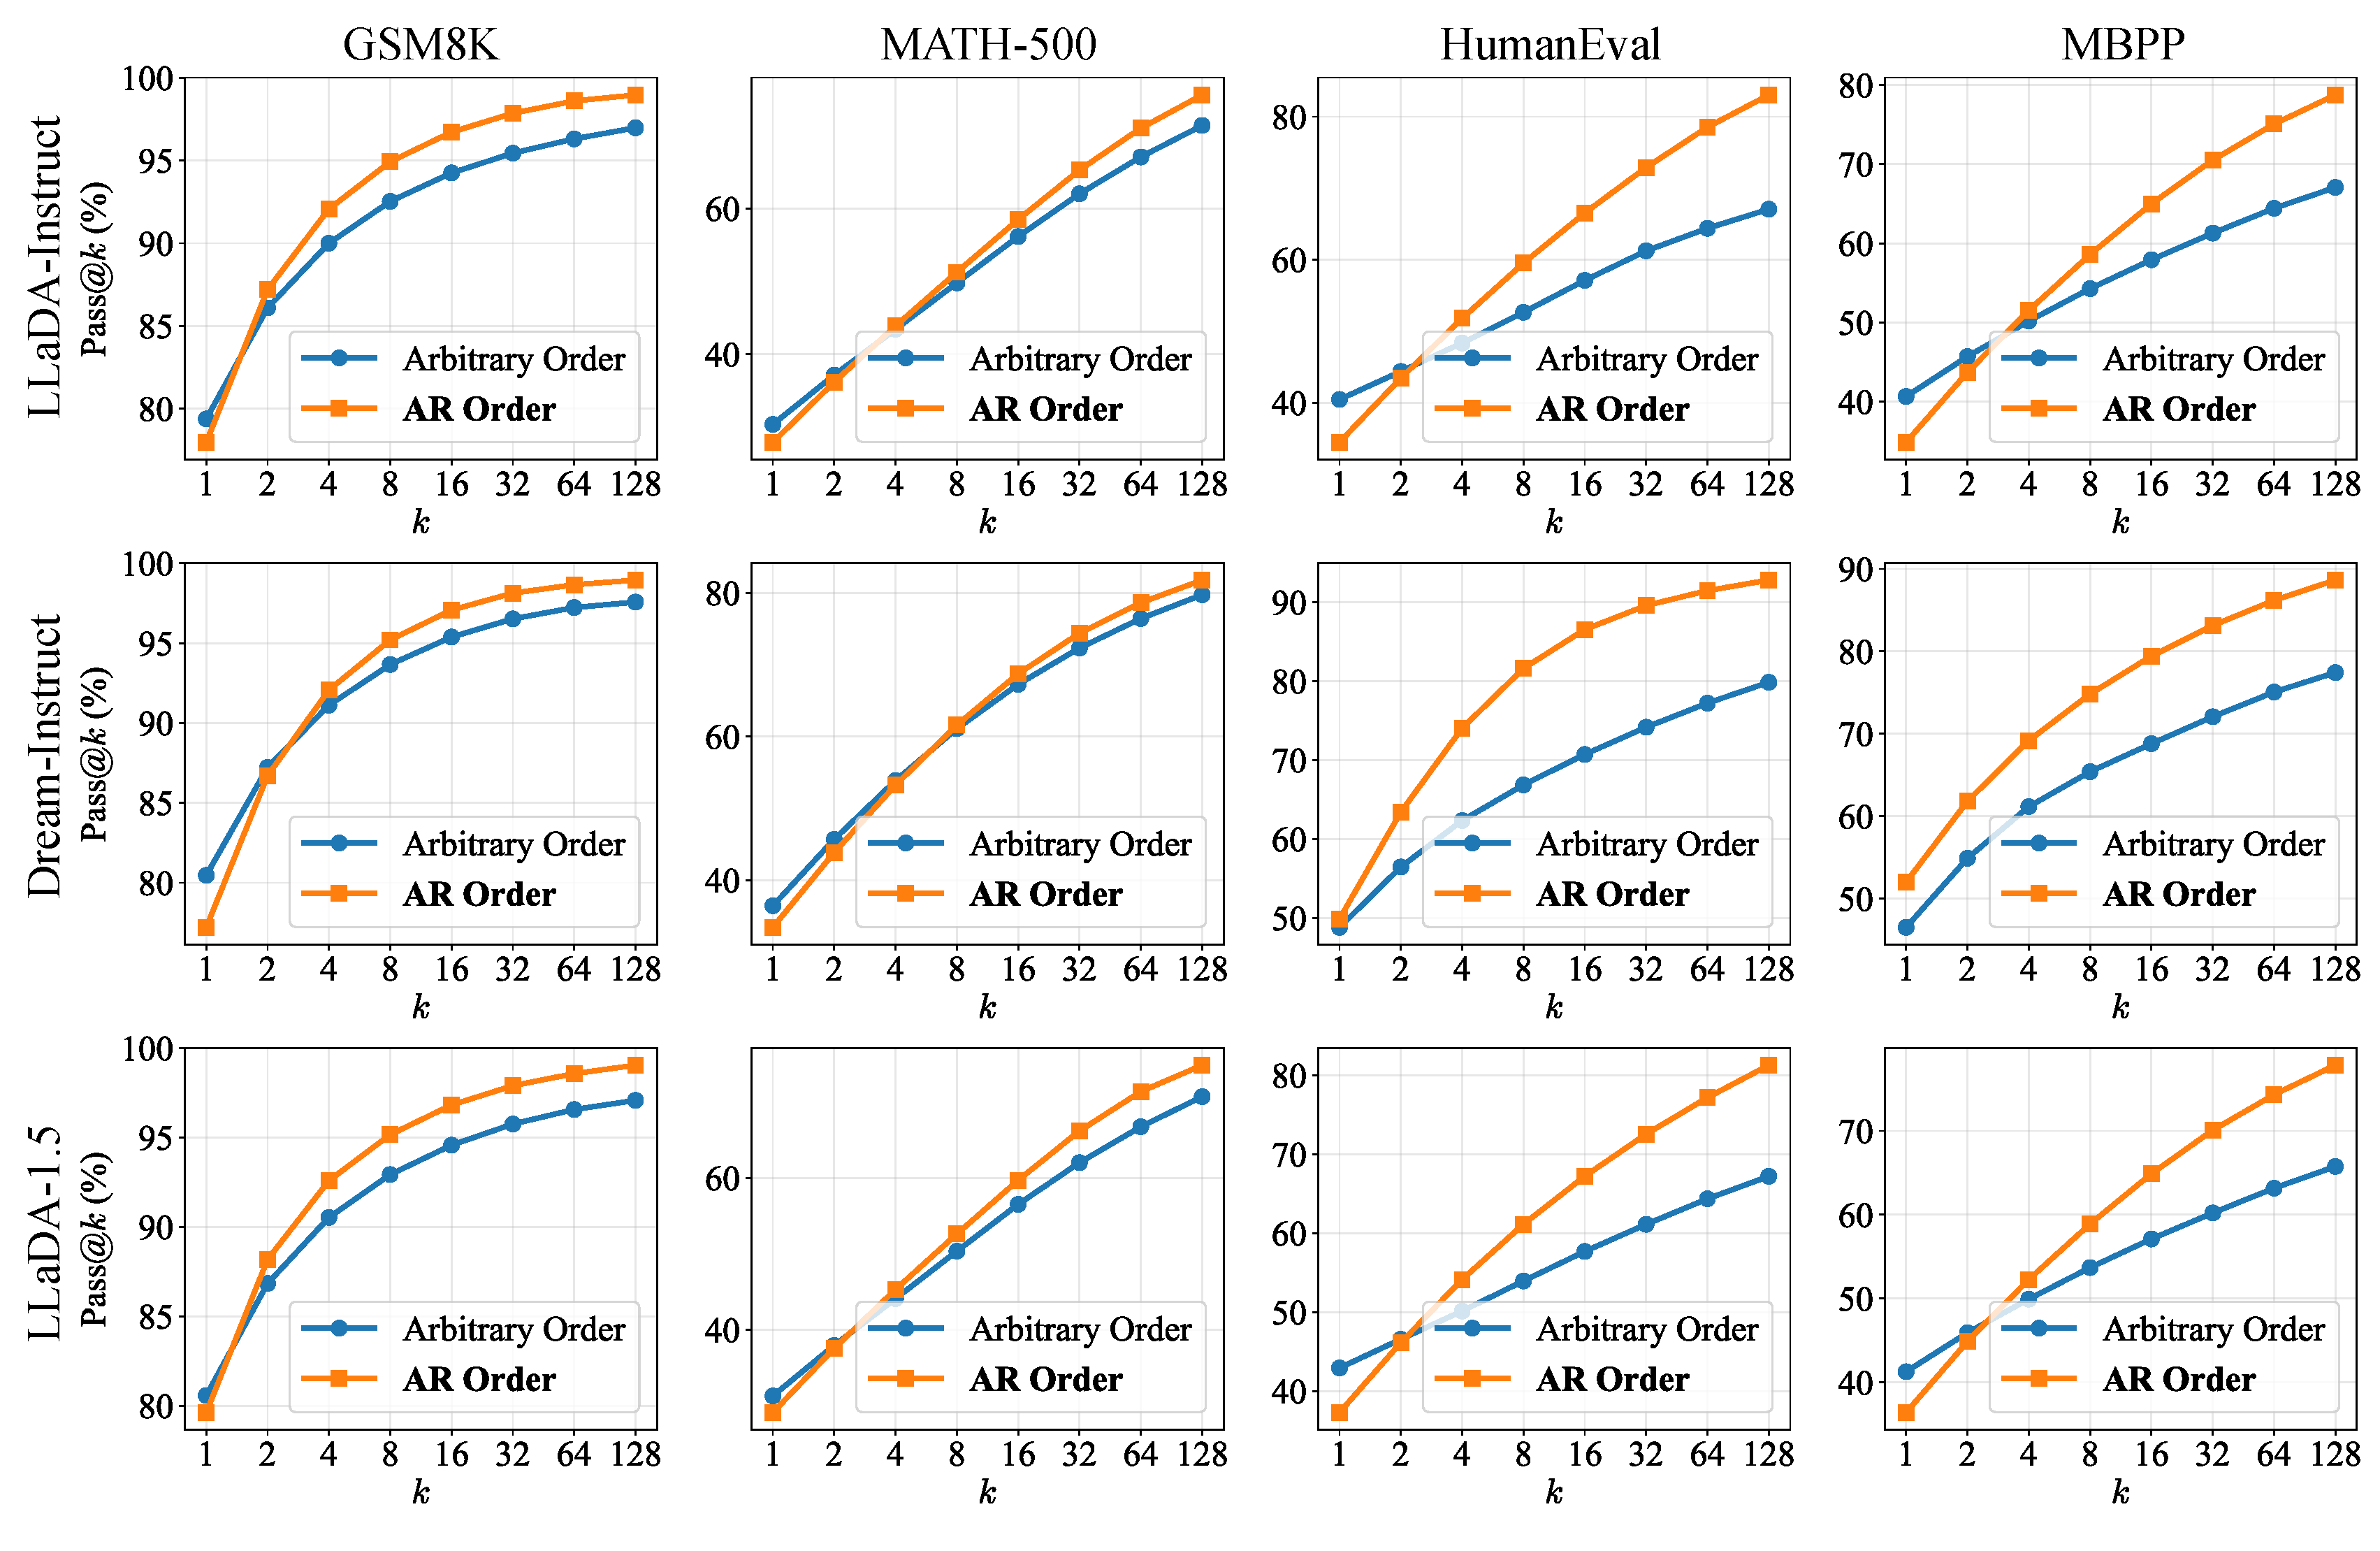
\includegraphics[width=\linewidth]{figures/passk_comparison.pdf}
\vskip -.15in
\caption{
    \textbf{Pass@$k$로 측정한 reasoning 잠재력.} arbitrary order는 single-shot 설정($k=1$)에서 경쟁력이 있지만, AR Order에 비해 더 평평한 scaling curves를 보인다.
    이러한 관찰은 서로 다른 dLLMs와 일반 reasoning benchmarks 전반에서 일관된다.
    \label{fig:passk_comparison}
}
\end{figure}

\begin{wrapfigure}{r}{0.52\textwidth}
    \centering
    \vskip -0.22in
    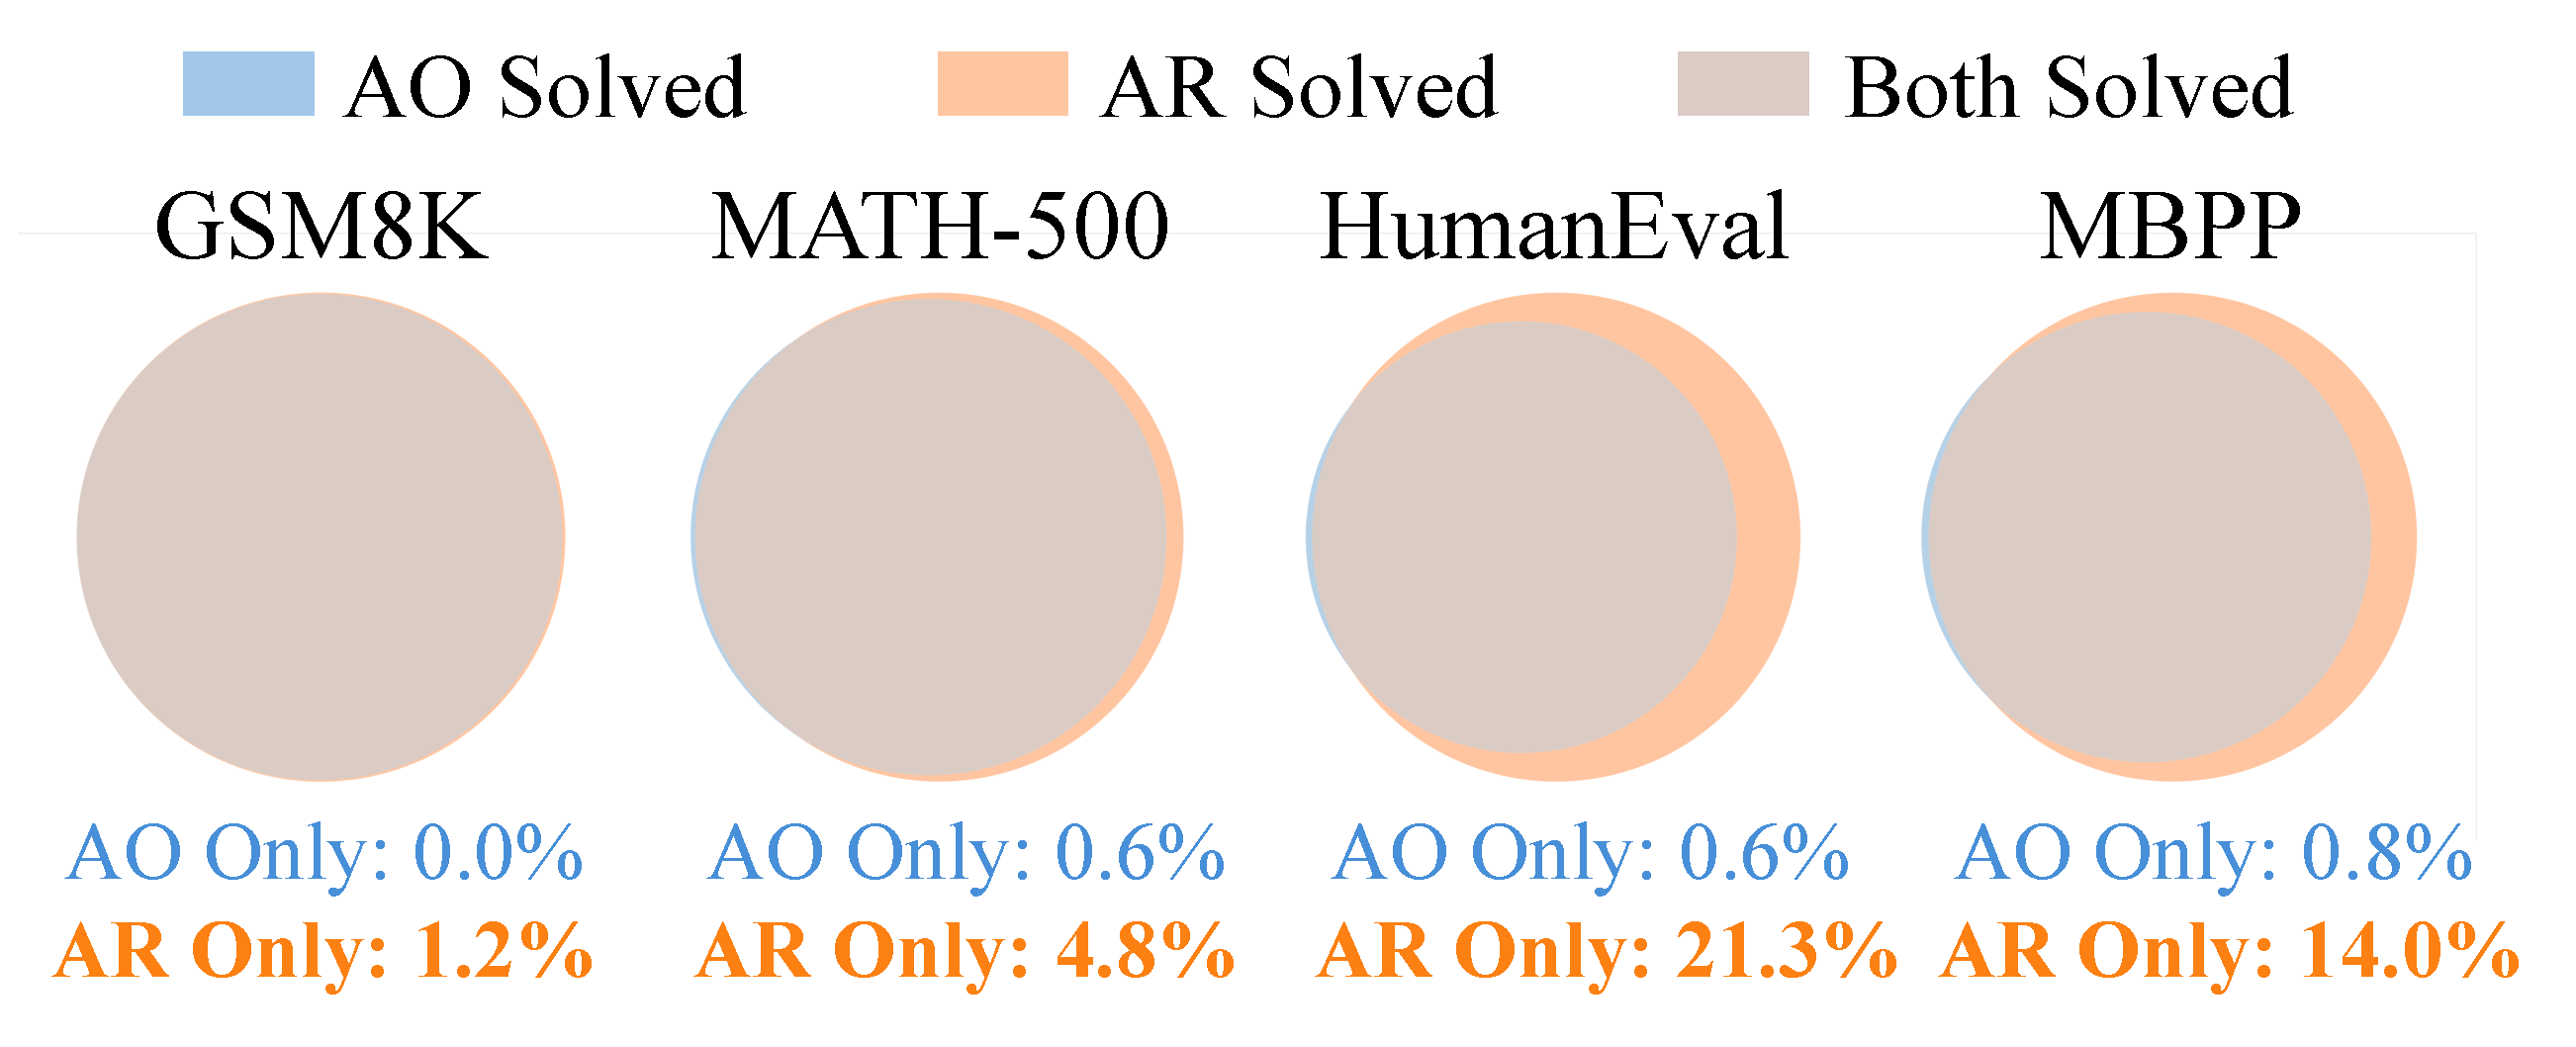
\includegraphics[width=\linewidth]{figures/venn.pdf}
    \vskip -.1in
    \caption{
        \textbf{Pass@$1024$로 측정한 solution space coverage.} arbitrary order (AO)로 풀 수 있는 문제들은 대체로 AR Order가 해결한 문제들의 subset이다.
        결과는 LLaDA-Instruct로 측정했다.
    }
    \label{fig:ar_vs_diff_venn}
    \vskip -0.18in
\end{wrapfigure}


\paragraph{Solution space coverage.}
arbitrary order가 효율은 낮더라도 다른 solution space를 탐색하며, 이것이 낮은 reasoning 잠재력을 설명할 수 있지 않을까 생각할 수 있다.
우리는 LLaDA-Instruct를 사용해 $k=1024$에서 solution coverage를 분석하여 이를 검증한다. 
Figure~\ref{fig:ar_vs_diff_venn}에 보이듯, arbitrary-order generation을 통해 얻은 solutions는 AR decoding이 발견한 solutions와 대체로 겹치며, 실제로는 더 작은 subset을 이룬다는 것을 발견했다.
예를 들어 HumanEval에서 문제의 21.3\%는 AR에 의해서만 해결되는 반면, 그 반대 경우는 드물다(0.6\%).
arbitrary-order generation은 이론적으로 더 큰 solution space를 함의하지만, 실제 sampling regime에서 효과적으로 도달 가능한 solution들의 집합은 더 제약적인 것으로 보인다.


\begin{wrapfigure}{r}{0.46\textwidth}
    \centering
    \vskip -0.28in
    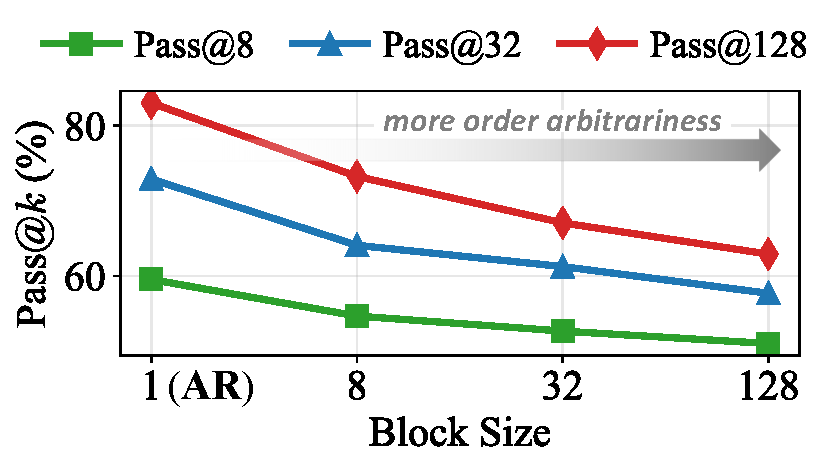
\includegraphics[width=\linewidth]{figures/block_size_humaneval.pdf}
    \vskip -0.15in
    \caption{
        \textbf{더 큰 arbitrariness, 더 낮은 potential.}
        우리는 서로 다른 수준의 order arbitrariness에 대해 semi-autoregressive decoding block size $B$를 sweep한다: $B=1$은 순수 AR order를 복원하고, 더 큰 $B$는 sampler가 다음에 어떤 position을 resolve할지 선택하는 데 더 많은 자유를 부여한다. 결과는 LLaDA-Instruct로 HumanEval에서 측정했다.
        \label{fig:arbitrary_block_size_analysis}
    }
    \vskip -0.4in
\end{wrapfigure}
\paragraph{더 큰 arbitrariness, 더 낮은 potential.}
지금까지 우리는 arbitrary order와 AR order를 두 극단으로 대비했지만, arbitrariness의 정도는 이분법적이지 않다. dLLMs~\cite{nie2025large,ye2025dream}의 semi-autoregressive protocol은 block size $B$를 통해 이를 제어한다: sequence는 크기 $B$의 blocks로 나뉘고, 각 block 안에서 model은 unmask할 tokens를 adaptive하게 선택한다.
따라서 $B$는 model이 다음 position을 자유롭게 선택할 수 있는 범위를 정하며, $B=1$은 자유도를 남기지 않고(순수 AR order) 더 큰 $B$는 더 arbitrary한 decoding을 허용한다; 위의 실험에서는~\cite{zhao2025d1}를 따라 $B=32$를 사용했다.
이제 $B$를 sweep하여 arbitrariness의 정도가 reasoning 잠재력에 어떤 영향을 미치는지 조사한다.

Figure~\ref{fig:arbitrary_block_size_analysis}에 보이듯, 추세는 일관되고 단조롭다: 모든 $k \in \{8, 32, 128\}$에 걸쳐 $B$가 커질수록 Pass@$k$는 감소한다. 이는 그 효과가 두 극단적 설정에 묶인 것이 아니라 일관적임을 시사한다: 이 설정에서는 더 낮은 arbitrariness가 더 높은 reasoning 잠재력과 일관되게 연관된다.

\subsection{Mechanism: Entropy Degradation}


\begin{wrapfigure}{r}{0.30\textwidth}
    \centering
    \vskip -0.15in
    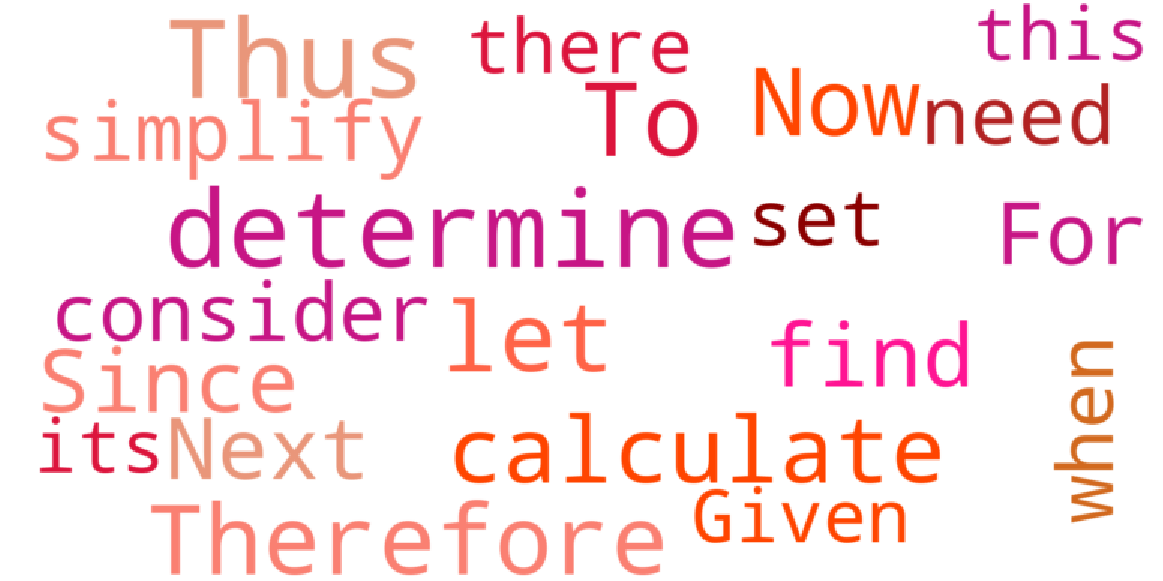
\includegraphics[width=\linewidth]{figures/bypass_words.pdf}
    \vskip -0.10in
    \caption{
        arbitrary order에서 \textbf{자주 bypass되는 tokens}는 보통 논리적 연결어와 전환어이다.
        결과는 LLaDA-Instruct로 MATH-500에서 측정했다.
        \label{fig:bypass_words}
    }
    \vskip -0.14in
\end{wrapfigure}
\paragraph{Adaptive decoding은 logical forks를 bypass한다.}
dLLMs의 이론적으로 더 큰 solution space가 실제로는 왜 collapse되는지 이해하기 위해, 두 decoding 모드가 어떻게 작동하는지 더 자세히 살펴본다.
AR order에서 model은 각 step마다 가장 왼쪽의 unknown token을 엄격히 resolve하도록 제약되어, uncertainty가 발생하는 순간 이를 직면하게 된다.
반대로 arbitrary order는 model confidence를 바탕으로 update할 tokens를 \emph{adaptive하게} 선택하며, ``어려운'' ones를 bypass하는 동안 높은 certainty를 가진 ``쉬운'' tokens를 우선적으로 생성한다.
자주 bypass되는 tokens를 살펴보면 명확한 pattern이 드러난다:
Figure~\ref{fig:bypass_words}에 보이듯, diffusion sampler는 ``Therefore'', ``Thus'', ``Since''와 같은 논리적 접속어와 전환 표지를 불균형적으로 뒤로 미룬다.
기존 연구는 그러한 tokens가 종종 높은 entropy를 가지며(dLLMs에서도 마찬가지이다; Figure~\ref{fig:bypass_compare} 참조), 이후 reasoning 방향을 결정하는 분기점으로 기능하는 ``reasoning sparks'' 또는 ``logical forks''로 작용한다는 것을 보였다~\cite{wang2025beyond,cheng2025reasoning,huang2025low}.
기존 language models에서는 이러한 tokens를 high-entropy state로 유지하는 것이 reasoning space의 효과적인 exploration에 중요하다~\cite{wang2025beyond}.

\begin{wrapfigure}{r}{0.5\linewidth}
    \centering
    \vskip -0.2in
    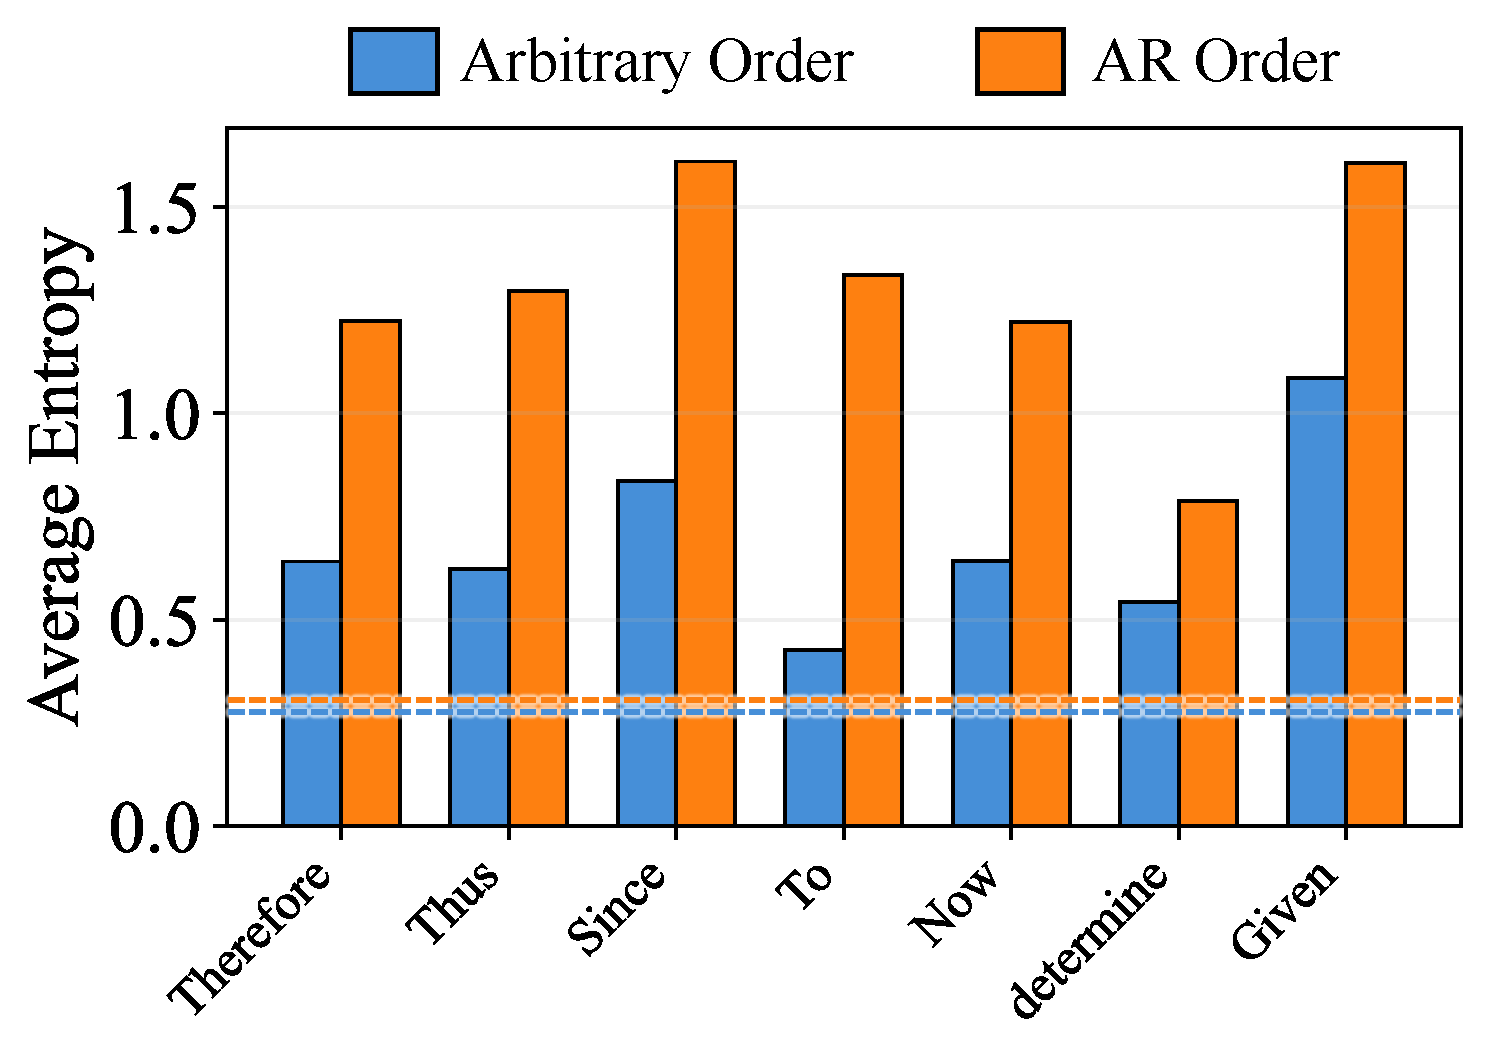
\includegraphics[width=\linewidth]{figures/entropy_bar_compare.pdf}
    \vskip -0.06in
    \caption{
        \textbf{Entropy degradation.} arbitrary order의 global average token entropy(점선)는 AR과 비슷한 수준을 유지하지만, logical forks(파란 막대)에서의 entropy는 크게 감소한다.
        결과는 LLaDA-Instruct로 MATH-500에서 측정했다.
        \label{fig:bypass_compare}
    }
    \vskip -0.14in
\end{wrapfigure}
\paragraph{``entropy degradation'' 현상.}
arbitrary order의 adaptive behavior는 이러한 logical forking tokens에 어떤 영향을 미치는가?
우리는 Figure~\ref{fig:bypass_compare}에서 이 tokens가 decoded될 때의 entropy를 측정한다(더 많은 결과는 Appendix~\ref{app:more_results_entropy_degradation}).
AR order에서는 이러한 tokens가 decoding될 때 일반적으로 높은 entropy를 유지하는데, 이는 여러 reasoning paths가 여전히 viable한 비교적 풍부한 branching point를 나타낸다~\cite{wang2025beyond}.
반대로 arbitrary order는 entropy의 급격한 감소를 보인다.
logical connectors를 뒤로 미룸으로써, model은 그들로 이어지는 logic connections를 결정하기 \emph{전에} 더 쉬운 future tokens 생성을 우선시한다.
model이 결국 bypass된 connectors를 채우기 위해 돌아오면, future context의 존재가 uncertainty를 크게 줄인다.
그 결과 model은 fork에서 open-ended navigational decision을 내리는 것이 아니라, 미리 정해진 conclusion으로 이어지는 gap을 bridge하기 위한 retrospective alignment에 가까운 일을 하게 된다.
우리는 이 현상을 \emph{entropy degradation}이라고 부른다.

\paragraph{Conclusion.}
요약하면, 우리의 발견은 일반 reasoning tasks에서 arbitrary order의 유연성이 inference-time exploitation을 exploration보다 의도치 않게 선호하게 만들 수 있음을 시사한다.
관찰된 entropy degradation은 이러한 경향의 정량적 지표 역할을 한다: uncertainty가 낮은 결정을 우선함으로써, model은 generation process의 초기에 자신의 trajectory를 특정 outcomes에 암묵적으로 anchor한다.
이는 solution space를 효과적으로 제약하여, single-shot coherence는 더 높일 수 있지만 complex problem-solving에 필요한 넓은 exploration을 제한할 수 있다.
표준 AR ordering은 causal chain을 엄격히 따름으로써 logical forks의 high-entropy 성질을 유지한다.
중요한 decision points를 우회할 수 없다는 점은 model이 다양한 reasoning branches에서 sample하도록 장려하며, 이는 reinforcement learning에 필수적인 solution coverage를 보존하는 데 도움이 된다.

\section{dLLMs를 위한 ``Just GRPO''}
\label{sec:justgrpo}

Section~\ref{sec:rethink_value_of_AO}의 발견은 arbitrary order가 RL이 접근할 수 있는 reasoning 잠재력을 제한할 수 있음을 시사한다. 그럼에도 현재 dLLMs를 위한 RL 방법들은 이 특정 유연성을 보존해야 한다는 필요에 여전히 크게 부담을 지고 있다.
이 절에서는 이 유연성이 부과하는 ``tax''를 검토하고(Section~\ref{sec:justgrpo_revisit}), 이를 포기하면 minimalist하면서도 효과적인 solution인 \textbf{JustGRPO}가 가능해짐을 보인다(Section~\ref{sec:justgrpo_detail}).

\subsection{dLLMs의 RL에서 Flexibility Tax}
\label{sec:justgrpo_revisit}
기존 diffusion RL 방법들은 arbitrary order generation을 보존하기 위해 policy가 denoising trajectories $\mathcal{T}$의 조합적 space를 수용해야 한다는 전제 아래 작동한다. 이 design choice는 개념적으로 일반적이지만, 몇 가지 challenges를 도입한다:

\paragraph{Token-level decomposition의 ambiguity.}
dLLMs에서 generation state $s_t$는 stochastic unmasking trajectory $\tau$에 condition된 noisy sequence이다.
autoregressive models와 달리, dLLMs는 $\pi(o_t \mid s_t)$ 형태의 고유하고 index-aligned된 conditional probability를 허용하지 않으므로, token-level credit assignment가 모호해지고 표준 importance ratio $\rho_t = \frac{\pi_\theta(o_t \mid s_t)}{\pi_{\text{old}}(o_t \mid s_t)}$를 정의하기 어렵게 만든다.

\paragraph{다루기 어려운 sequence likelihood.}
Autoregressive models는 sequence likelihood를 $\log \pi(o) = \sum_t \log \pi(o_t \mid o_{<t}, q)$로 factorize하는 반면, dLLMs는 모든 valid denoising trajectories에 대한 marginalization을 요구한다,
$\pi_\theta(o \mid q) = \sum_{\tau \in \mathcal{T}} \pi_\theta(o, \tau \mid q)$.
길이 $N$의 sequence에 대해 trajectory space는 $|\mathcal{T}| = O(N!)$로 증가하여, exact likelihood computation을 infeasible하게 만들고 기존 방법들이 original objective 대신 ELBO 기반 surrogate에 의존하도록 강제한다~\cite{wang2025spg,ou2025principled}.

\paragraph{Sampler-learner mismatch.}
정확한 likelihood approximation이 있더라도, 더 subtle한 문제가 남아 있다.
실제로 rollout samples는 조합적 space를 탐색하기 위해 보통 \emph{confidence-based} generation $o \sim \pi_{\theta}^{\text{conf}}(o \mid q)$로 생성된다.
그러나 ELBO objective는 여전히 실제 sampling policy $\pi_{\theta}^{\text{conf}}(o \mid q)$가 아니라 \emph{original} model distribution $\pi_\theta(o \mid q)$의 likelihood를 목표로 하며, 이는 rollout과 optimization 사이의 mismatch를 초래하여 성능을 저하시킬 수 있다~\cite{schulman2015trust}.


\subsection{JustGRPO}
\label{sec:justgrpo_detail}
우리는 단순함으로 돌아갈 것을 제안한다. 우리의 분석에서 순수 autoregressive order가 더 높은 reasoning 잠재력을 보이므로(Section~\ref{sec:rethink_value_of_AO}), RL stage 동안 arbitrary-order generation을 명시적으로 포기한다. 이 constraint는 dLLM을 혼란스러운 sequence denoiser에서 잘 정의된 autoregressive policy로 변환한다.

\paragraph{Formulation.}
Standard GRPO는 모든 tokens가 observed된 \emph{partial} sequence $o_{<k}$를 받아들이고 한 번에 \emph{one} token $o_k$를 예측하는 policy $\pi(o_k | o_{<k}, q)$를 가정하며, 여기서 $q$는 query이다.
그러나 diffusion language models는 observed tokens와 masked tokens가 섞인 \emph{full} sequence를 받아들이고 모든 masked positions의 original values를 동시에 예측하는 sequence-level denoisers로 설계되어 있다.

arbitrary-order generation을 포기함으로써, 우리는 위의 gap을 bridge하고 dLLMs에 대한 AR policy $\pi_{\theta}^{\text{AR}}$를 엄밀하게 정의할 수 있다.
history $o_{<k}$가 주어졌을 때 next token $o_k$의 probability를 얻기 위해, past는 observed되고 future는 masked된 $\tilde{x}_k$를 구성한다:
\begin{equation}
    \tilde{x}_k = [\underbrace{o_1, \dots, o_{k-1}}_{\text{Observed}}, \underbrace{\texttt{[MASK]}, \dots, \texttt{[MASK]}}_{\text{Masked}}].
\end{equation}
diffusion language model은 모든 masked positions에 대한 predictions를 출력하지만, autoregressive policy는 next token $o_k$에만 관심을 둔다. 우리는 $\pi_{\theta}^{\text{AR}}(\cdot | o_{<k}, q)$를 다음과 같이 정의한다:
\begin{equation}
    \pi_{\theta}^{\text{AR}}(\cdot | o_{<k}, q) \triangleq \text{Softmax}(f_{\theta, k}(\tilde{x}_k, q)),
\end{equation}
여기서 $f_{\theta, k}$는 position $k$에서의 model logits를 나타낸다.
dLLM backbone 위에 surrogate autoregressive policy $\pi_{\theta}^{AR}$를 정의함으로써, 우리는 permutations에 대한 다루기 어려운 marginalization을 정확하게 계산 가능한 likelihood로 변환한다:
\begin{equation}
    \pi_{\theta}^{\text{AR}}(o | q) = \prod_{k=1}^{|o|} \pi_{\theta}^{\text{AR}}(o_k | o_{<k}, q).
\end{equation}

\paragraph{Optimization.}
위 formulation은 standard GRPO를 diffusion language models에 직접 적용할 수 있게 한다. 각 query $q$에 대해, 우리는 old policy $\pi_{\theta_{\text{old}}}^{\text{AR}}$를 사용해 outputs group $\{o_i\}_{i=1}^G$를 sample한다. objective는 다음과 같다:
\begin{equation}
    \label{eq:justgrpo-loss}
    \mathcal{J}(\theta) = \mathbb{E}_{q \sim P(Q), \{o_i\}_{i=1}^G \sim \pi_{\theta_{\text{old}}}^{\text{AR}}} \Bigg[ \frac{1}{G} \sum_{i=1}^G \frac{1}{|o_i|} \sum_{k=1}^{|o_i|} \Big( \min \big( \rho_{i,k} \hat{A}_{i,k}, \text{clip}(\rho_{i,k}, 1-\varepsilon, 1+\varepsilon) \hat{A}_{i,k} \big) - \beta \mathbb{D}_{\text{KL}} \Big) \Bigg],
\end{equation}
여기서 $\rho_{i,k} = \frac{\pi_\theta^{\text{AR}}(o_{i,k} \mid o_{i,<k}, q)}{\pi_{\theta_{\text{old}}}^{\text{AR}}(o_{i,k} \mid o_{i,<k}, q)}$는 current policy와 old policy 사이의 probability ratio이고, $\hat{A}_{i,k}$는 group-standardized advantage를 나타낸다.

\paragraph{Remarks.}
AR mode에서 training하는 것이 diffusion model을 fundamentally standard autoregressive model로 바꾸는 것은 아닌지 우려할 수 있다. 
그렇지 않다. AR constraint는 더 효과적인 exploration과 credit assignment를 위해 \emph{RL training 동안에만} 적용된다.
중요하게도, 이는 underlying structure를 바꾸거나 dLLMs 고유의 parallel sampling을 훼손할 수 있는 structural constraints, \eg, causal masking을 부과하지 않고 model distribution을 정제한다.
경험적으로 model은 inference에서 decoding을 가속하기 위해 parallel samplers~\cite{ben2025accelerated}와 계속 compatible하다. 따라서 JustGRPO는 dLLMs의 parallel capability를 보존하면서 AR 기반 reasoning exploration의 이점을 얻는다(Section~\ref{subsec:parallel_decoding} 참조).


\section{실험}
\label{sec:experiments}

우리는 표준 mathematical reasoning 및 coding benchmarks에서 JustGRPO를 평가한다. 우리의 실험 설계는 두 가지 가설을 검토하는 것을 목표로 한다. (i) RL training 동안 autoregressive (AR) order를 강제하면 복잡한 arbitrary-order approximation에 의존하지 않고도 reasoning capabilities를 효과적으로 끌어낼 수 있다는 점, (ii) 이 제약은 최적화 objective에만 적용되어 inference 시 diffusion model의 parallel decoding capabilities는 그대로 유지된다는 점이다.

\begin{table}[t]
    \centering
    \caption{LLaDA-Instruct에서 post-training approaches의 \textbf{system-level comparison}. JustGRPO는 단순함에도 강한 성능을 달성한다.
    Baseline 수치는 대부분 각 원 논문에서 인용했다\protect\footnotemark{}.
    이러한 baselines 사이에서 실험 설정이 완전히 일관되지는 않음을 밝혀 둔다. JustGRPO는 모든 tasks에서 full fine-tuning을 사용하고 step마다 하나의 token을 unmask한다. Baseline 중 LLaDA-1.5, LLaDOU, ESPO도 step마다 하나의 token을 unmask하는 반면, 나머지는 step마다 두 개의 token을 unmask한다. LLaDA-1.5와 LLaDOU도 full fine-tuning을 사용하고, ESPO는 code tasks에서만 그렇게 하며(그 외에는 LoRA), 나머지는 LoRA를 사용한다.
    이러한 이질성을 고려하여, 원래 설정이 우리와 다른 몇 가지 대표 baseline을 Table~\ref{tab:controlled_comparison}에서 통일된 protocol 아래 추가로 재현했으며, 여기에서도 동일한 결론이 유지된다.
    \label{tab:main_results}}
    \vskip -.05in
    \renewcommand{\arraystretch}{1.08}
    \resizebox{\linewidth}{!}{
        \begin{tabular}{l ccc ccc ccc ccc}
            \toprule
            & \multicolumn{3}{c}{\textbf{GSM8K}}
            & \multicolumn{3}{c}{\textbf{MATH-500}}
            & \multicolumn{3}{c}{\textbf{HumanEval}}
            & \multicolumn{3}{c}{\textbf{MBPP}} \\
            \cmidrule(lr){2-4}
            \cmidrule(lr){5-7}
            \cmidrule(lr){8-10}
            \cmidrule(lr){11-13}
            \textbf{Model / Seq Len }
            & \textbf{128} & \textbf{256} & \textbf{512}
            & \textbf{128} & \textbf{256} & \textbf{512}
            & \textbf{128} & \textbf{256} & \textbf{512}
            & \textbf{128} & \textbf{256} & \textbf{512} \\
            \midrule
            d1~\cite{zhao2025d1}
            & 73.2 & 81.1 & 82.1
            & 33.8 & 38.6 & 40.2
            & - & - & -
            & - & - & - \\
            LLaDOU$^\dagger$~\cite{huang2025reinforcing}
            & - & 88.1 & -
            & - & 41.1 & -
            & - & \textbf{59.1} & -
            & - & 51.6 & - \\
            LLaDA-1.5$^\ddagger$~\cite{zhu2025llada}
            & - & 83.3 & -
            & - & - & -
            & 29.3 & 39.6 & \textbf{51.9}
            & 39.6 & 39.9 & 38.8 \\
            wd1~\cite{tang2025wd1}
            & 77.2 & 80.8 & 82.3
            & 33.3 & 34.4 & 39.0
            & - & - & -
            & - & - & - \\
            $d$-TreeRPO~\cite{pan2025d}
            & - & 81.2 & 82.6
            & - & 37.7 & 38.9
            & - & - & -
            & - & - & - \\
            ESPO~\cite{ou2025principled}
            & 80.0 & 82.3 & 83.7
            & 36.0 & 39.0 & 43.4
            & 28.1 & 42.1 & 50.0
            & 47.4 & 44.6 & 44.2 \\
            GDPO~\cite{rojas2025improving}
            & 78.4 & 82.8 & 84.5
            & 33.2 & 39.6 & 41.4
            & 26.2 & 39.6 & 39.0
            & 43.6 & 50.6 & 47.1 \\
            SPG~\cite{wang2025spg}
            & 78.5 & 86.1 & 84.5
            & 33.4 & 40.0 & 41.8
            & - & - & -
            & - & - & - \\
            \midrule
            \textbf{JustGRPO}
            & \textbf{83.8} & \textbf{89.1} & \textbf{89.8}
            & \textbf{39.0} & \textbf{45.1} & \textbf{45.2}
            & \textbf{37.8} & 49.4 & 48.7
            & \textbf{50.6} & \textbf{52.4} & \textbf{49.0} \\
            \bottomrule
        \end{tabular}
    }
    \par\vskip 2pt
    \noindent\parbox{\linewidth}{\footnotesize\raggedright
        $^\dagger$ LLaDOU는 auxiliary module로 base architecture를 수정한다.\\
        $^\ddagger$ LLaDA-1.5는 훨씬 더 큰 규모의 비공개 수집 dataset에서 학습된다.}
    \vskip -.05in
\end{table}

\footnotetext{두 가지 예외가 있다. LLaDOU의 MATH-500 결과($41.1$)는 원 논문이 MATH-500이 아니라 전체 MATH test set을 보고하기 때문에 우리가 official checkpoint로 측정했다. LLaDA-1.5 수치는~\cite{ou2025principled}에서 가져왔다.}

\paragraph{실험 설정.}
우리는 LLaDA-Instruct~\cite{nie2025large}에 JustGRPO를 적용하고, 네 가지 표준 reasoning 및 coding benchmarks인 GSM8K, MATH-500, HumanEval, MBPP에서 그 효과를 평가한다.
Mathematical tasks의 경우~\cite{zhao2025d1,ou2025principled}를 따라 각 dataset의 official training split으로 학습한다. Coding tasks의 경우 AceCoder-87K~\cite{zeng2025acecoder}의 subset으로~\cite{gong2025diffucoder,ou2025principled}를 따라 학습한다.
우리는 추가 task-specific SFT 없이 full-parameter fine-tuning을 사용해 JustGRPO를 모델에 직접 적용한다.
우리의 training recipe는 대체로~\cite{huang2025reinforcing}를 따른다.
학습된 모델을 평가하기 위해 표준 LLaDA evaluation protocol~\cite{nie2025large}을 따르며, 이는 32-token block에서 semi-autoregressive decoding과 함께 low-confidence remasking을 적용한다(step마다 하나의 token을 unmask, \ie, generation length 256의 경우 256 steps). Sampling temperature는 0을 사용한다.
우리는~\cite{zhao2025d1,ou2025principled}를 따라 generation length 128, 256, 512에서 모든 benchmarks를 평가한다.
Training에 대한 자세한 내용은 Appendix~\ref{app:experimental_setups}에 제공된다.

\subsection{주요 결과}
\label{subsec:main_results}

\paragraph{Reasoning tasks에서의 성능.} Table~\ref{tab:main_results}는 system-level comparison을 보고한다. 우리는 diffusion-specific RL adaptation이 전혀 필요 없음에도 표준 GRPO 정식화를 단순히 적용하는 것만으로 이미 강한 전반적 성능을 달성함을 관찰한다. GSM8K에서 JustGRPO는 89.1\% accuracy(seq len 256)에 도달하여 이전 diffusion-specific methods와 경쟁적이거나 더 높으며, 더 어려운 MATH-500에서도 유사한 경향을 보인다. 또한 auxiliary trainable module이나 더 큰 규모의 private training data를 활용하고 HumanEval에서 더 높은 accuracy를 보고하는 LLaDOU 및 LLaDA-1.5와도 전반적으로 경쟁력을 유지한다.
\begin{wraptable}{r}{0.58\textwidth}
    \centering
    \vskip -0.15in
    \caption{\textbf{우리 설정과 정렬된 configurations에서의 재현} (full fine-tuning, decoding step마다 하나의 token, generation length 256). 재현한 baselines는 $^{*}$로 표시했다. HumanEval 및 MBPP의 ESPO$^{*}$ 결과는 원 논문에서 직접 가져왔으며, 해당 설정은 이미 우리와 일치한다(full fine-tuning, decoding step마다 하나의 token).}
    \vskip -0.12in
    \label{tab:controlled_comparison}
    \small
    \setlength{\tabcolsep}{4pt}
    \begin{tabular}{lcccc}
        \toprule
        \textbf{Model} & \textbf{GSM8K} & \textbf{MATH-500} & \textbf{HumanEval} & \textbf{MBPP} \\
        \midrule
        d1$^{*}$           & 83.8 & 39.2 & -- & -- \\
        ESPO$^{*}$         & 84.7 & 40.3 & 42.1 & 44.6 \\
        SPG$^{*}$          & 86.9 & 41.8 & -- & -- \\
        \textbf{JustGRPO}  & \textbf{89.1} & \textbf{45.1} & \textbf{49.4} & \textbf{52.4} \\
        \bottomrule
    \end{tabular}
    \vskip -0.12in
\end{wraptable}
Table~\ref{tab:main_results}의 수치는 이질적인 설정에서 paper-reported된 것이므로(캡션 참조), 우리는 우리와 정렬된 통일 protocol(full-parameter fine-tuning, decoding step마다 하나의 token, generation length 256) 아래 대표 baseline들을 추가로 재현한다.
Table~\ref{tab:controlled_comparison}에 보이듯, JustGRPO는 이 비교에서도 여전히 앞서며, 이는 denoising trajectories의 전체 조합 공간 위에서 최적화하는 것이 반드시 필요하지 않을 수 있고, training 동안 dLLM을 sequential generator로 취급하는 것이 일반 reasoning tasks에 단순하지만 효과적인 recipe라는 관점과 일치한다.

\subsection{JustGRPO는 Parallel Decoding을 보존한다}
\label{subsec:parallel_decoding}

\begin{figure}[t]
    \centering
    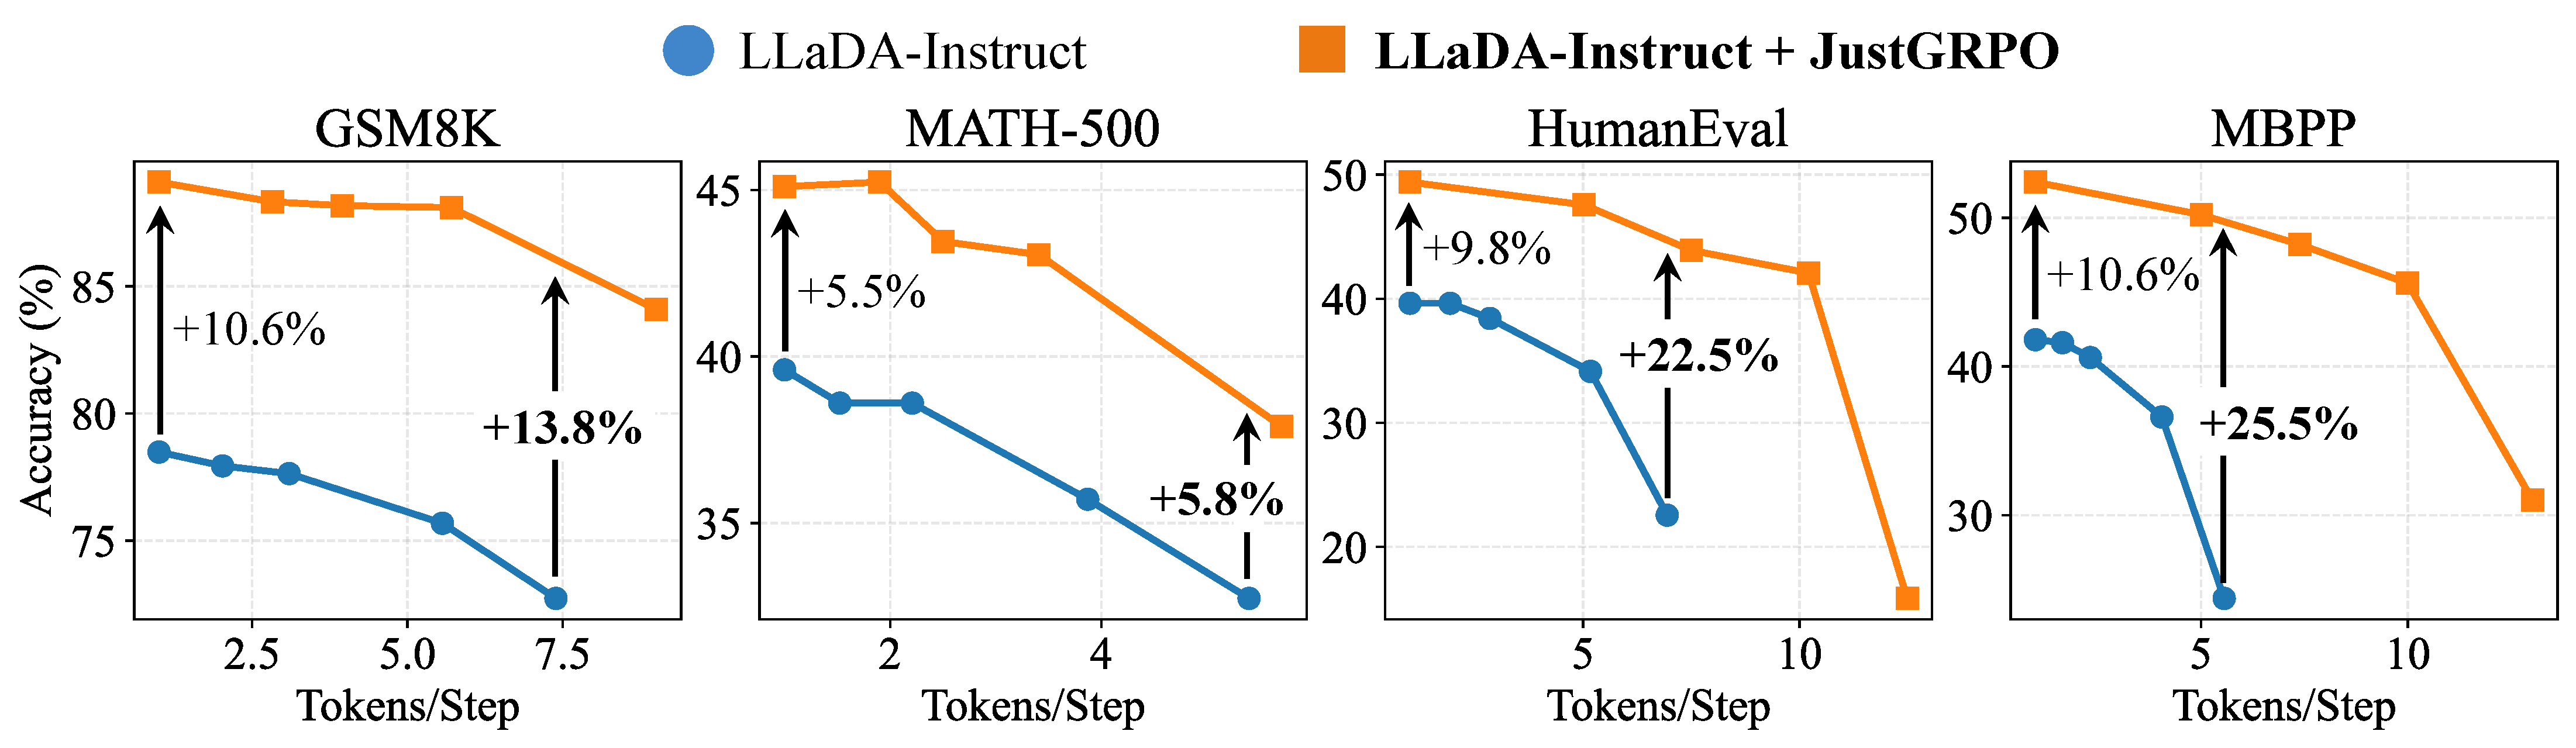
\includegraphics[width=.95\linewidth]{figures/parallel.pdf}
    \vskip -.1in
    \caption{\textbf{JustGRPO는 dLLM의 parallel decoding capability를 보존한다.}
    흥미롭게도 original instruct model과 비교하면, parallel tokens가 많을수록 accuracy gains가 더 커지는데, 이는 JustGRPO training 후 reasoning capabilities가 더 robust해졌기 때문일 가능성이 있다.
    우리는 parallel decoding을 위해 training-free EB-sampler~\cite{ben2025accelerated}를 채택한다. Generation length는 256으로 설정한다.
    }
    \label{fig:eb_sampler_comparison}
    \vskip -.05in
\end{figure}

우리는 AR training이 dLLM의 parallel decoding capabilities를 저해하는지 추가로 조사한다. Training-free Entropy Bounded (EB) Sampler~\cite{ben2025accelerated}를 사용하여 다양한 병렬성 수준(tokens per step)에서 inference performance를 평가한다.

Figure~\ref{fig:eb_sampler_comparison}는 우리 모델이 parallel decoding과 완전한 호환성을 유지하며 original LLaDA-Instruct model에 비해 speed와 accuracy 사이에서 유리한 trade-off를 보임을 보여 준다. 흥미롭게도 parallelism이 증가할수록 성능 이득은 더 두드러진다.
Baseline의 성능은 high parallel steps에서 급격히 저하되는 반면, 우리 모델은 상대적으로 더 안정적인 성능을 유지한다. 예를 들어 MBPP에서 accuracy gap은 보수적 설정(1 token/step)의 +10.6\%에서 공격적 설정($\sim$5 tokens/step)의 +25.5\%로 확대된다.
이는 특정 trajectory에 overfitting하기보다, AR formulation이 underlying model distribution을 정련하는 효과적인 training ``scaffold'' 역할을 할 수 있음을 시사한다.
이렇게 정련된 분포는 original model에 비해 parallel sampling에 내재한 approximation에 더 탄력적인 것으로 보인다.


\subsection{Training Efficiency}
\label{subsec:efficiency}

\begin{wrapfigure}{r}{0.4\textwidth}
    \centering
    \vskip -0.12in
    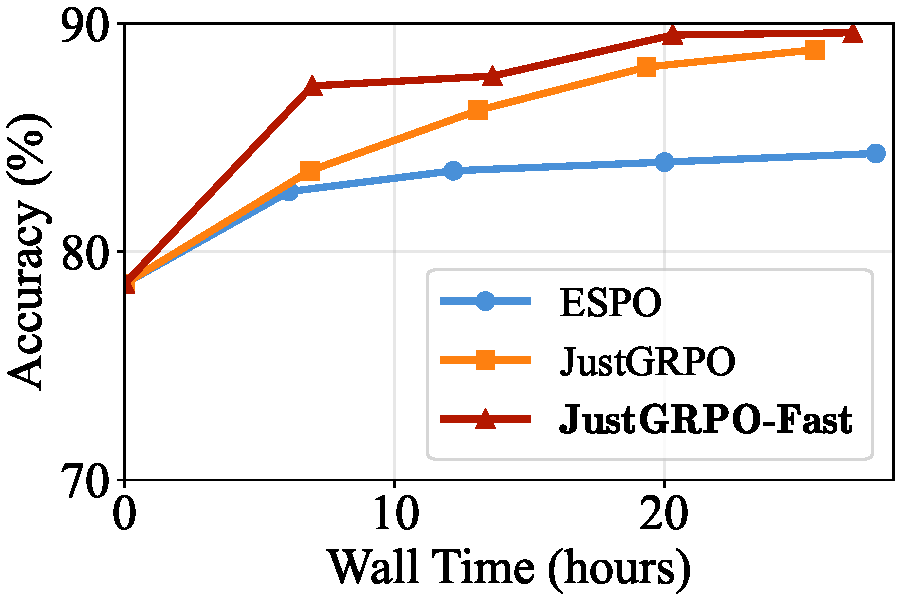
\includegraphics[width=\linewidth]{figures/gsm8k_walltime.pdf}
    \vskip -.05in
    \caption{\textbf{GSM8K에서의 training efficiency.} Iteration당 overhead가 더 큼에도, JustGRPO는 일찍 포화되는 approximation-based baseline(ESPO)보다 더 나은 accuracy/wall-time trade-off를 달성한다. JustGRPO-Fast는 가장 entropy가 높은 상위 25\% positions에서만 probability ratio $\rho_{i,k}$를 계산하여 training을 더욱 가속한다. Wall time은 16$\times$H100 GPUs에서 측정했다.}
    \label{fig:walltime_efficiency}
    \vskip -0.14in
\end{wrapfigure}
Exact GRPO를 dLLM에 적용하는 것은 구조적 trade-off를 수반한다. Autoregressive models와 달리 dLLM은 single causal forward pass가 아니라 각 position을 독립적으로 평가해야 하므로, exact likelihood를 계산하면 iteration당 추가 overhead가 발생한다. 이전 방법들~\cite{zhao2025d1,ou2025principled}은 approximation에 의존하여 이 비용을 우회했으며, 이는 비교상 exact optimization이 비실용적일 수 있음을 시사하는 듯하다. 그러나 Figure~\ref{fig:walltime_efficiency}는 그렇지 않음을 시사한다. 이러한 overhead가 있더라도 JustGRPO는 accuracy/wall-clock trade-off에서 경쟁력을 유지하며, 대표적인 approximation-based baseline(ESPO)의 peak accuracy를 비슷한 시간 안에 맞추고 계속 향상된다.

더욱이 이 overhead는 근본적인 것이 아니다. 지배적인 원인은 GRPO objective(Eq.~\ref{eq:justgrpo-loss})에서 per-position probability ratios $\rho_{i,k}$를 계산하는 데 있다. Reasoning이 sparse set of high-entropy forking tokens에 의해 조향된다는 우리의 발견(Section~\ref{sec:rethink_value_of_AO})에 동기를 얻어, 우리는 가장 entropy가 높은 상위 25\% positions에서만 $\rho_{i,k}$를 평가하여 이러한 forward evaluations의 75\%를 제거하는 JustGRPO-Fast를 도입한다.

중요하게도 per-token entropy는 rollout stage 동안 직접 기록할 수 있으므로, high-entropy positions를 식별하는 데 드는 overhead는 무시할 만하다. 경험적으로 JustGRPO-Fast는 기본 JustGRPO보다도 accuracy/wall-time trade-off를 개선하며, 기본 JustGRPO 자체도 이미 approximation-based baseline(ESPO)보다 유리하고 더 짧은 wall-clock time 안에 비슷한 accuracy에 도달한다.



\section{관련 연구}
\label{sec:related}


\paragraph{Diffusion language models.} 
연속 영역에서 diffusion model이 거둔 성공~\cite{ho2020denoising,rombach2022high}에 동기를 얻어, 최근 연구들은 diffusion을 이산 텍스트 생성으로 확장했다. 초기 embedding-space 접근법~\cite{diffusionlm,diffuseq,ssdlm}은 최적화와 이산화 문제에 직면했고, 이에 따라 random masking을 통해 이산 토큰 공간에서 직접 작동하는 masked diffusion model~\cite{sedd,mdlm,shi2024simplified,ou2024your}이 채택되었다.
LLaDA~\cite{nie2025large}와 Dream~\cite{ye2025dream} 같은 최근의 대규모 모델은 autoregressive (AR) 모델과 경쟁할 만한 성능을 달성한다.
문헌에서 논의된 dLLM의 여러 장점 가운데 두 가지 측면이 특히 주목받았다. 첫째, dLLM은 본질적으로 parallel decoding을 지원하여 상당한 inference 가속을 가능하게 한다~\cite{fastdllm,ben2025accelerated,labs2025mercury,geminidiffusion,song2025seed}. 둘째, dLLM의 non-autoregressive 정식화는 arbitrary-order 토큰 생성을 허용하며, 이는 엄격한 left-to-right 제약을 완화함으로써 복잡한 reasoning에 도움이 될 수 있다고 가정되어 왔다~\cite{ye2024beyond,kim2025train}.

\paragraph{순서 임의성의 가치.} 초기 연구들이 제한된 과제에서 arbitrary order 생성을 검증한 반면~\cite{ye2024beyond,nie2025large,kim2025train}, 최근 연구는 이를 일반 reasoning으로 확장한다. 일부 연구는 dLLM이 자연스럽게 비표준 decoding 동작(\eg, sketch-first)을 보일 수 있음을 입증하고~\cite{xie2025dream,gong2025diffucoder}, 다른 연구는 성능 향상을 위해 decoding schedule을 명시적으로 최적화한다~\cite{Peng2025PathPF,huang2025reinforcing}.
또한 일부 연구~\cite{gong2025diffucoder,hong2025improving,shen2026improvingdiffusionlanguagemodel}는 dLLM의 reasoning 잠재력을 측정하기 위해 Pass@$k$도 사용한다.
이 잠재력을 인식한 이러한 연구들은 주로 arbitrary-order 패러다임 안에서 성능을 높이는 데 초점을 맞추며, 그 이점이 순서 임의성에 고유하게 묶여 있는지는 덜 검토된 채로 남겨 두었다.
최근 \cite{du2025understanding}는 arbitrary order의 필요성에 의문을 제기하며, 모델이 uniform permutation을 학습하도록 강제하면 기저 데이터 분포에 대한 근사가 상당히 느슨해진다고 주장했다.
그들의 분석은 pre-training에 초점을 두지만, 우리는 reasoning과 RL에서도 유사한 failure mode를 관찰하며, 이러한 유연성이 RL training에 필수적인 exploration을 저하시킬 수 있음을 시사한다.
이는 sequence의 ordering이 그 내용뿐 아니라 유용한 구조적 정보도 담고 있으며 arbitrary-order 생성은 이를 간과하기 쉽다는 더 넓은 관점~\cite{varshney2006toward}과도 관련된다.

\paragraph{Diffusion language model을 위한 reinforcement learning.} dLLM을 위한 reinforcement learning은 autoregressive 패러다임과 구별되는 구조적 최적화 장애물에 직면하며, 이는 주로 denoising trajectory의 조합적 폭발에서 비롯된다. 초기 시도들~\cite{zhao2025d1,yang2025mmada,gong2025diffucoder}은 token-level 정식화를 직접 적용하려 했지만, ill-defined state transition으로 인해 종종 제한되었고 mean-field approximation에 의존할 필요가 있었다. 그 결과 이 분야는 sequence-level 관점~\cite{wang2025spg,rojas2025improving,ou2025principled}으로 이동하여, 다루기 어려운 marginal likelihood를 근사하기 위한 다양한 surrogate를 사용하게 되었다. 그러나 이러한 방법 전반에는 off-policy misalignment가 종종 남아 있다. 효율적인 exploration에 필요한 heuristic-guided sampling이 기저 diffusion prior에서 벗어나며, 이는 원칙적인 보정 없이 gradient에 편향을 줄 수 있기 때문이다~\cite{schulman2015trust}.
두 가지 주목할 만한 예외는 이러한 문제를 부분적으로 다룬다. LLaDOU~\cite{huang2025reinforcing}는 토큰 위치 선택을 모델링하기 위한 auxiliary policy를 도입하여 직접적인 trajectory likelihood 추정을 가능하게 하고, TraceRL~\cite{wang2025revolutionizing}은 shrinkage-based step-wise MDP를 통해 최적화를 inference trace와 정렬한다. 그럼에도 둘 다 전체 arbitrary-order 메커니즘을 유지하며 그 필요성을 암묵적으로 가정하는 반면, 우리는 arbitrary order 자체의 필요성을 재고함으로써 효과적인 RL training을 더 단순하게 달성할 수 있는지 질문한다.

\section{결론}
\label{sec:conclusion}
Diffusion language model의 직관적 매력은 순서 임의성에 있으며, 이는 종종 복잡한 reasoning 경로를 탐색하기 위한 유망한 메커니즘으로 여겨진다. 그러나 우리의 연구는 수학과 코딩 같은 일반 reasoning tasks에서 이러한 제한 없는 유연성이 오히려 reasoning 잠재력을 의도치 않게 제약할 수 있음을 시사한다.
구체적으로, arbitrary-order 생성은 더 넓은 solution coverage보다 단일 trajectory의 refinement를 우선시하는 것으로 보인다.

이 관찰은 dLLM의 reasoning capabilities를 끌어내기 위한 더 단순한 해법을 가리킨다. 표준 autoregressive objective를 사용해 모델을 정렬함으로써, 우리는 order arbitrariness에 맞춘 복잡한 adaptation 없이 Group Relative Policy Optimization (GRPO)을 직접 적용할 수 있게 한다. 이 접근법인 JustGRPO는 단순함에도 불구하고 training 동안 exploration order를 의도적으로 제약하는 것이 reasoning performance의 주목할 만한 향상을 가져올 수 있으며, inference에서는 dLLM의 parallel decoding capabilities를 완전히 보존한다는 점을 시사한다. 정렬을 위해 기본적인 left-to-right order로 돌아감으로써, 본 연구는 diffusion language model 개발에서 arbitrary \emph{vs.} AR order 사이의 trade-off를 재고하도록 한다.


\section*{영향 진술}
이 논문은 Machine Learning 분야, 특히 diffusion language model과 reasoning task를 위한 reinforcement learning 영역을 발전시키는 것을 목표로 하는 연구를 제시한다. 우리의 발견은 더 단순한 학습 접근법이 놀라울 정도로 효과적일 수 있음을 시사하며, 이는 계산 비용을 줄이고 이러한 기법의 접근성을 높일 수 있다. 본 연구에는 여러 잠재적인 사회적 영향이 있을 수 있지만, 주요 기여가 방법론적이며 language model의 이해와 학습을 개선하는 데 목적을 두고 있으므로 여기서 특별히 강조해야 할 사항은 없다고 본다.

\section*{감사의 말}
이 연구는 중국 국가 중점 R\&D 프로그램(Grant 2024YFB4708200), 중국 국가 자연과학기금(Grants U24B20173, U2541227, 625B2107), 그리고 청년 교원을 위한 과학연구 혁신역량 지원 프로젝트(Grant ZYGXQNJSKYCXNLZCXM-I20)의 부분적 지원을 받았다.

\bibliography{main}
\bibliographystyle{icml2025}


\newpage
\appendix
\section*{Appendix}
\label{sec:appendix}

\section{실험 세부사항}
\label{app:experimental_setups}

\subsection{Data Preparation}
Mathematical reasoning tasks의 경우, 표준 protocol~\cite{zhao2025d1,ou2025principled}을 따라 각 dataset의 official training split으로 학습한다.
Code generation tasks의 경우, AceCoder-87K dataset~\cite{zeng2025acecoder}을 채택한다. DiffuCoder~\cite{gong2025diffucoder}의 data processing pipeline을 따라, 검증 가능한 unit tests가 갖춰진 AceCoder-87K의 challenging samples 21K개를 추가로 선택한다.

\subsection{Training Configuration}
우리의 training setup은 대체로~\cite{huang2025reinforcing}를 따른다.
\cite{huang2025reinforcing}와 달리, 우리는 추가 trainable modules를 도입하지 않고 dLLM에 직접 reinforcement learning을 수행한다.
Rollout phase 동안에는 exact autoregressive sampling을 채택하며, 이는 표준 GRPO formulation 아래 직접적인 log-probability 계산을 가능하게 한다.
또한 JustGRPO가 빠르고 안정적인 convergence를 보이므로 training steps의 총수도 줄인다.
모든 실험은 16$\times$ NVIDIA H100 GPUs에서 수행된다. 자세한 hyperparameters는 Table~\ref{tab:hyperparams}에 보고한다.


\begin{table}[H]
    \centering
    \caption{JustGRPO의 \textbf{training hyperparameters}\protect\footnotemark{}.}
    \label{tab:hyperparams}
    \begin{tabular}{lc}
        \toprule
        \textbf{Hyperparameter} & \textbf{Value} \\
        \midrule
        Base Model & LLaDA 8B Instruct \\
        RL Algorithm & GRPO \\
        Optimizer & AdamW \\
        Learning Rate & $5 \times 10^{-6}$ \\
        LR Scheduler & Constant \\
        Weight Decay & 0.0 \\
        Optimizer Betas $(\beta_1, \beta_2)$ & $(0.9, 0.999)$ \\
        Global Batch Size & 64 \\
        Group Size ($G$) & 16 \\
        Policy Update Steps & 1 \\
        Training Steps & 125 \\
        Max Completion Length & 256 \\
        Sampling Temperature & 1.0 \\
        KL Penalty Coefficient & 0.0 \\
        \bottomrule
    \end{tabular}
\end{table}

\footnotetext{경험적으로 GSM8K는 훨씬 더 빠르게 convergence한다(약 50 steps에서 이미 $\sim$89\% accuracy에 도달). 반면 coding tasks(HumanEval, MBPP)는 더 느리며 전체 125 steps의 이점을 얻는다. 따라서 일관성을 위해 모든 datasets에 대해 125 steps를 동일하게 사용했다.
}
\subsection{Reward Function}
\label{app:reward_function}

\paragraph{Mathematical Reasoning Tasks.}
우리는 binary reward scheme을 사용한다. 각 completion은~\cite{huang2025reinforcing}를 따라 final answer가 ground-truth solution과 수학적으로 동등할 때에만 1의 reward를 받는다.

\paragraph{Code Generation Tasks.}
Code generation의 경우, total reward $r$은 correctness reward $r_{\text{code}}$와 format reward $r_{\text{format}}$의 합으로 정의된다.
\begin{equation}
    r = r_{\text{code}} + r_{\text{format}}.
\end{equation}

\begin{itemize}
    \item \textbf{Correctness reward ($r_{\text{code}}$)}: 제공된 unit tests에서 생성된 code의 pass rate(0에서 1 사이)로 정의된다. 이 항은 $r_{\text{format}} = 1$일 때에만 평가된다.
    \item \textbf{Format reward ($r_{\text{format}}$)}: 문법적으로 유효한 outputs을 장려하도록 설계된 heuristic reward이다.
    \begin{itemize}
        \item $1.0$: 올바른 Python syntax를 가진 유효한 Markdown code block.
        \item $0.5$: Syntax errors를 포함하지만 유효한 Markdown code block.
        \item $0.0$: 유효한 Markdown code block 생성 실패.
    \end{itemize}
\end{itemize}


\section{Reasoning Boundary에 대한 추가 분석 결과}
\label{app:boundary_ablations}
Section~\ref{sec:rethink_value_of_AO}에서 제시한 reasoning boundary에 관한 발견의 robust성을 추가로 검증하기 위해, LLaDA-Instruct model~\cite{nie2025large}을 사용하여 HumanEval benchmark에서 확장 분석을 수행한다. Temperature와 sampling strategies가 reasoning performance에 미치는 영향을 조사한다.

\subsection{Temperature Analysis}
\label{app:temperature_analysis}
\begin{figure}[ht]\centering
    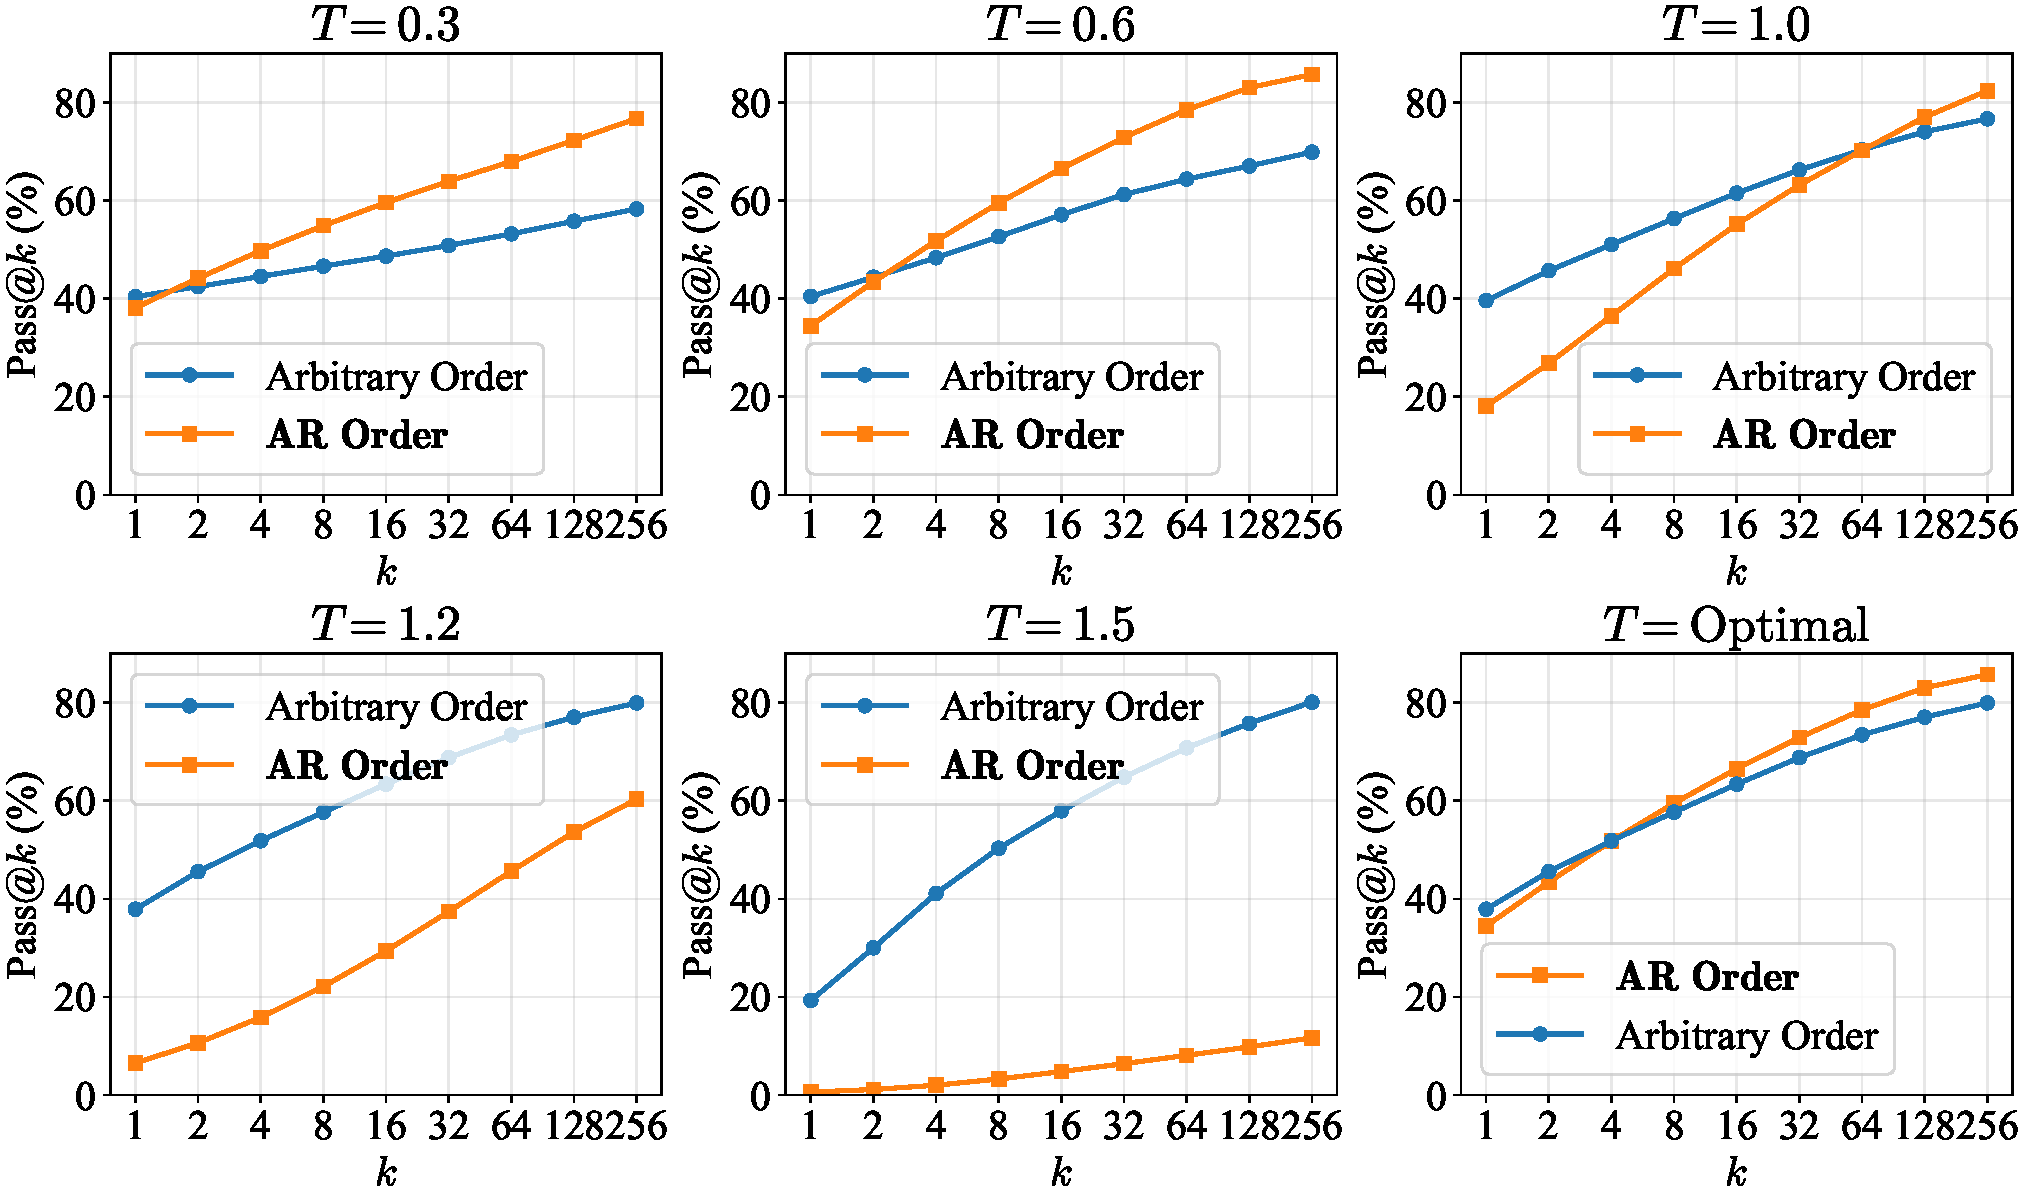
\includegraphics[width=.75\linewidth]{figures/humaneval_temp.pdf}
    \caption{
        \textbf{서로 다른 temperatures에서의 Pass@$k$ comparison\label{fig:passk_comparison_temperature}}.
    }
\end{figure}

HumanEval에서 우리는 Pass@$k$ plot을 $k=256$까지 확장한다. $1.0$에 가까운 temperatures에서는 두 modes 사이의 crossover가 비교적 큰 $k$에서 발생하며, 더 큰 budget은 그 이후의 비교를 검토할 수 있게 한다.
\cref{fig:passk_comparison_temperature}에 보이듯, AR mode는 표준적인 패턴을 보인다. 성능은 moderate temperatures($T \approx 0.6$)에서 peak에 도달하고 $T > 1.0$일 때 저하되는 반면, Arbitrary Order mode는 더 높은 temperatures에서 peak performance를 달성한다.

이 관찰은 Section~\ref{sec:rethink_value_of_AO}에서 논의한 \textit{entropy degradation} 메커니즘과 일치한다. Diffusion sampler가 critical branching points에서 본질적으로 uncertainty를 억제하므로, 충분한 exploration을 유도하려면 더 높은 temperatures가 필요하다.
주목할 점은 이러한 optimized settings에서도 arbitrary order mode가 우리의 실험에서 AR mode의 reasoning potential에 미치지 못한다는 것이다.
\cref{fig:passk_comparison_temperature}의 ``Optimal'' comparison setting(오른쪽 아래)에 나타난 것처럼, best-performing AR configuration은 여전히 optimal arbitrary order baseline보다 더 나은 scaling behavior를 보인다. 그럴듯한 설명은 arbitrary order decoding에서 지나치게 높은 temperatures가 높은 결정성이 필요한 tokens(\eg, code syntax 또는 mathematical suffixes)에 noise를 주입하여 nonsensical outputs과 저하된 결과를 초래한다는 것이다~\cite{wang2025beyond,huang2025low}.

\subsection{Different Sampling Algorithms}
우리는 Figure~\ref{fig:alg_comparison}(a)에서 negative entropy sampling (Neg-Entropy) ~\cite{ye2025dream} 및 top-$k$ margin sampling (Margin) ~\cite{kim2025train} 같은 다양한 sampling algorithms도 실험한다.
\begin{figure}[t]\centering
    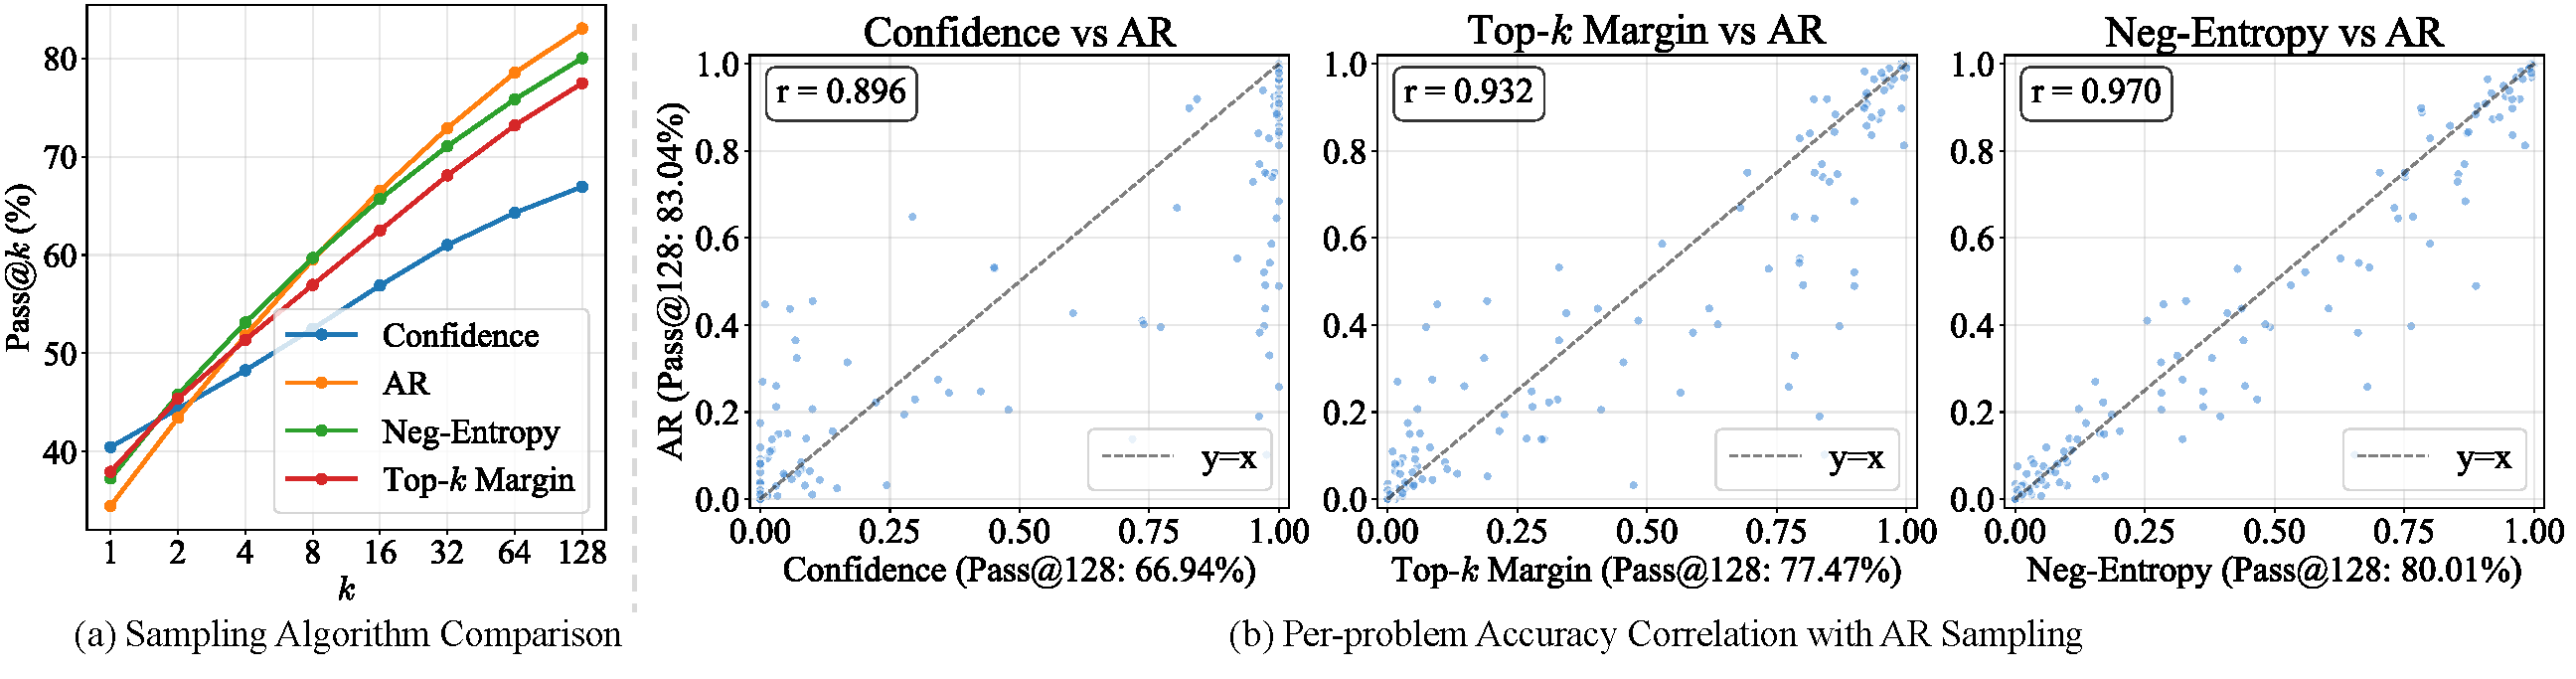
\includegraphics[width=\linewidth]{figures/alg_compare.pdf}
    \caption{
        \textbf{(a) Sampling algorithm comparison}.
        \textbf{(b) 서로 다른 sampling algorithms와 AR 사이의 per-problem accuracy 상관관계}.
        Pass@$k$ 성능이 더 높은 algorithms는 problem-level performance에서 \emph{AR과 더 높은 correlation}을 보이는 경향이 있다.
        \label{fig:alg_comparison}
    }
\end{figure}
결과는 더 정교한 sampling algorithms가 default confidence-based sampling보다 더 나은 Pass@$k$ 성능을 달성할 수는 있지만, 여전히 AR order를 따라잡지는 못함을 보여 준다.
한편 이러한 더 나은 Pass@$k$ algorithms는 confidence-based sampling에 비해 약간 더 낮은 Pass@$1$ 성능도 보이며, 전체 Pass@$k$ curve를 AR order의 Pass@$k$ curve에 더 가깝게 만든다.
이 유사성을 조사하기 위해 서로 다른 sampling algorithms와 AR mode 사이의 per-problem accuracy correlation을 계산한다(Figure~\ref{fig:alg_comparison}(b)).
우리는 더 높은 scaling potential(더 높은 Pass@$128$)을 가진 algorithms가 일관되게 AR과 더 강한 correlation을 보이며, 가장 효과적인 방법(Neg-Entropy)은 $0.970$의 correlation을 달성함을 관찰한다.
이는 더 나은 Pass@$k$를 가진 sampling algorithms가 performance characteristics에서 AR처럼 행동하는 경향이 있음을 시사한다.

\begin{figure}[ht]\centering
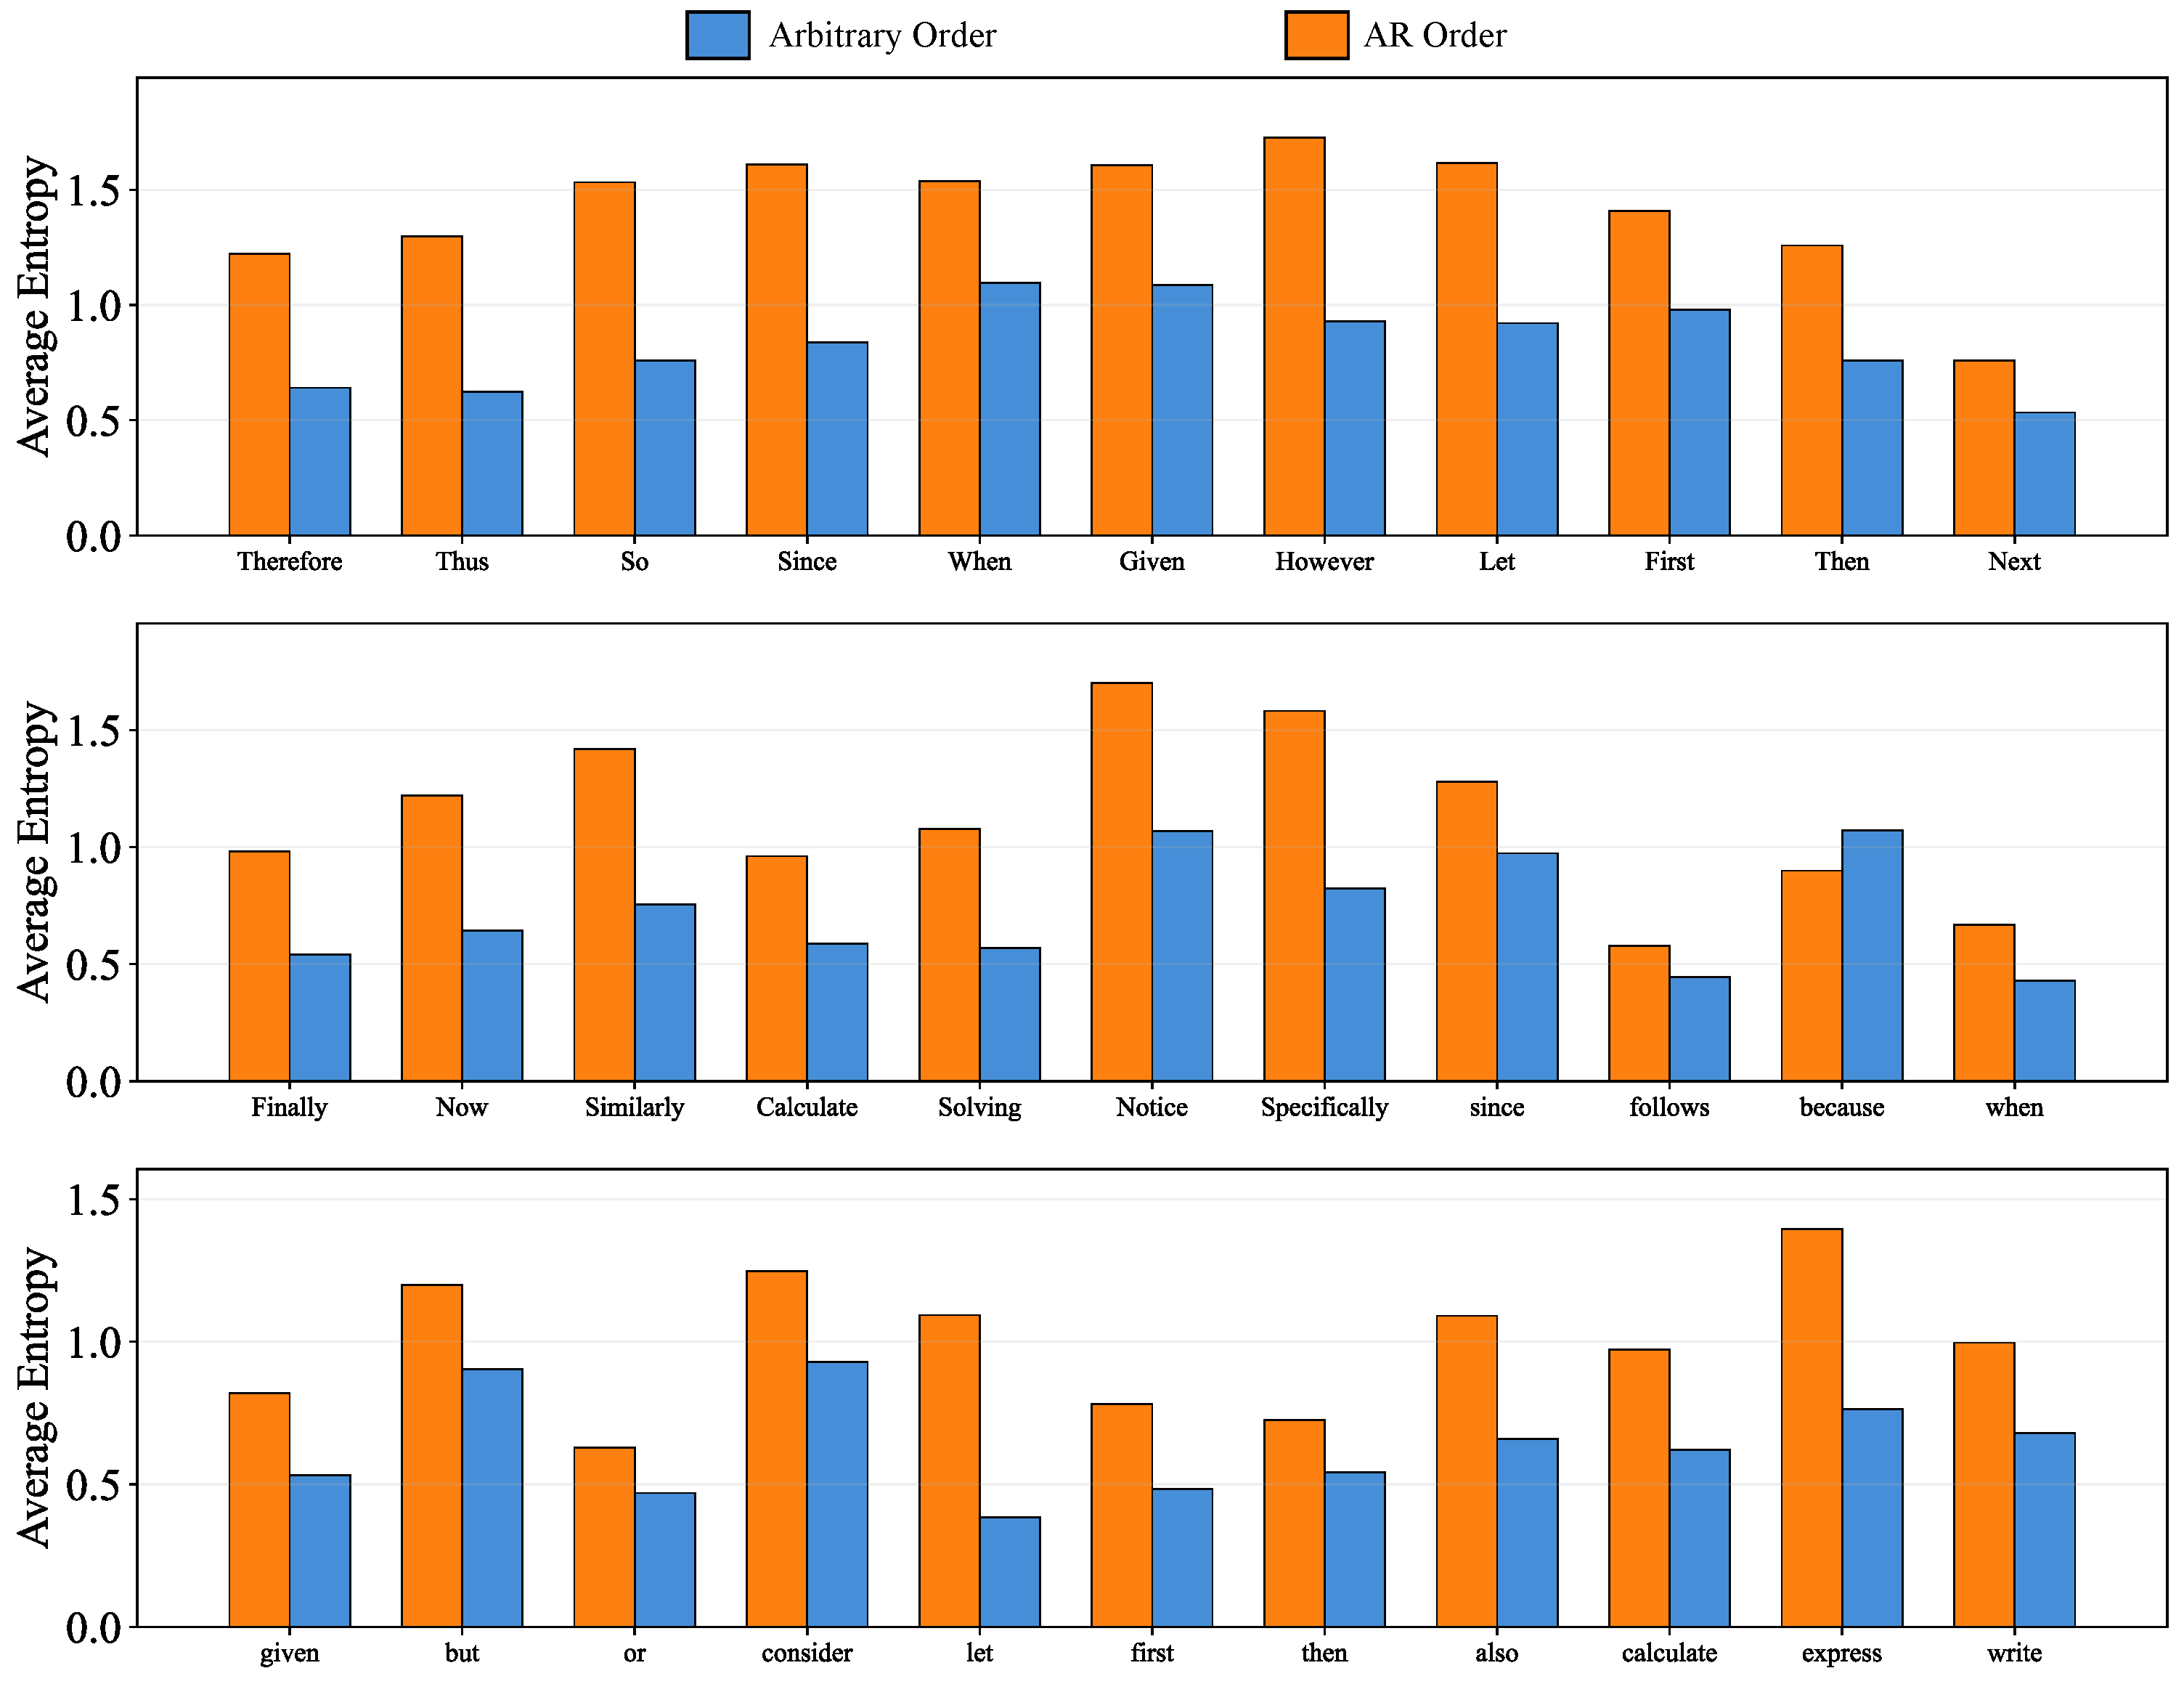
\includegraphics[width=\linewidth]{figures/entropy_bar_compare_more.pdf}
\caption{
    \textbf{더 많은 forking tokens에 대한 entropy comparison results\label{fig:entropy_bar_compare_more}}.
}
\end{figure}

\section{Entropy Degradation에 대한 추가 결과}
\label{app:more_results_entropy_degradation}

Section~\ref{sec:rethink_value_of_AO}에서 관찰한 ``entropy degradation'' 현상의 robust성을 검증하기 위해, 우리는 분석을 더 넓은 범위의 logical connectors로 확장했다. Reasoning chains에서 일반적으로 forking tokens로 작용하는 common connectives의 포괄적인 집합에 대해 실험을 수행했다.

\cref{fig:entropy_bar_compare_more}에 나타난 결과는 이 현상이 이러한 다양한 tokens 전반에서 일관됨을 보여 준다. 주요 발견과 유사하게, AR order는 이러한 forks에서 더 높은 average entropy를 유지하며, 이는 active reasoning과 decision-making을 나타낸다. 반대로 Arbitrary Order는 일관되게 더 낮은 entropy를 낳으며, branching possibilities의 premature collapse와 일치한다.

이 확장 실험에서 평가한 구체적인 forking tokens는 다음을 포함한다. ``Therefore'', ``Thus'', ``So'', ``Since'', ``When'', ``Given'', ``However'', ``Let'', ``First'', ``Then'', ``Next'', ``Finally'', ``Now'', ``Similarly'', ``Calculate'', ``Solving'', ``Notice'', ``Specifically'', ``Follows'', ``Because'', ``But'', ``Or'', ``Consider'', ``Also'', ``Express'', and ``Write''.



\section{Random Order는 대안인가?}
\label{app:random_order}

Section~\ref{sec:rethink_value_of_AO}의 우리의 주요 분석은 dLLM이 실제로 사용되는 방식, 즉 confidence-based sampling과 semi-autoregressive sampling~\cite{nie2025large,zhao2025d1}에 의해 decoding이 구동되는 설정에 관한 것이다. 이것이 bypassing이 발생하고 entropy가 degradation되는 설정이며, 우리의 분석이 겨냥하는 설정이다.

그러나 dLLM이 반드시 그러한 sampler를 사용해야 하는 것은 아니다. 자연스러운 질문은 original dLLM formulation~\cite{mdlm,shi2024simplified}과 연결되는 random decoding order가 다르게 행동할지 여부이다. 우리는 그것 역시 도움이 되지 않음을 발견한다.

\paragraph{Random order does not help coverage, and it breaks generation.}
Pass@$128$에서 random order는 기껏해야 confidence-based sampling과 비슷하며, 여전히 AR order에는 크게 못 미친다(Table~\ref{tab:random_passk}, 위). Pass@$1$은 훨씬 더 나빠서 두 baselines보다도 훨씬 낮다(Table~\ref{tab:random_passk}, 아래). 이유는 간단하다. dLLM에서 각 token은 주변 context로부터 예측되지만, random order는 종종 그 context가 존재하기 전에 모델이 token을 결정하도록 요구한다. 예를 들어 token~1만 알려진 상태에서 token~30을 예측하는 식이다. 그 결과 output은 단순히 틀리는 데 그치지 않고, 다음 LLaDA rollout이 보여 주듯 구조적으로 깨진다.

\begin{quote}
    \small\ttfamily
    3. **Third Month:**\\
    \ - The number of downloads reduced by 30\% compared to the second month.\\
    \ \textbackslash[ 180 - (\ \ \ \textbackslash times 180 - (\ \ \ - 180) = 180 - 0.30 \textbackslash times 180 = 54 \ldots \textbackslash]
\end{quote}

LaTeX가 손상되어 dangling operators와 missing operands가 생긴다. 이런 종류의 outputs은 reward를 얻는 경우가 드물며, 이는 RL이 학습할 수 있는 것을 제한한다.

\paragraph{Random order does not survive RL either.}
그 다음 random order를 우리의 training setup으로 가져온다. JustGRPO와 유사한 exact likelihood factorization을 적용하기 위해, 단일 random permutation을 채택하고 training 내내 고정한다. 우리는 이 variant를 JustGRPO-Random이라 부른다. Pipeline의 나머지는 그대로 유지했을 때, JustGRPO-Random은 GSM8K에서 82.2\%에만 도달하며, AR order의 89.1\%와 비교된다(Table~\ref{tab:random_order_ablation}). 따라서 random order는 remedy로 보이지 않는다. 우리의 실험에서 이는 sampler로서 coverage를 넓히지도 못하고 RL 이후 강한 reasoning을 제공하지도 못한다.

\begin{table}[H]
    \centering
    \caption{\textbf{Random order는 coverage를 개선하지 못하고 single-shot accuracy를 붕괴시킨다.} LLaDA-Instruct에서 측정한 confidence-based arbitrary order, fully random order, AR order의 Pass@$128$(위) 및 Pass@$1$(아래).}
    \label{tab:random_passk}
    \begin{tabular}{lcccc}
        \toprule
        \textbf{Method} & \textbf{GSM8K} & \textbf{MATH-500} & \textbf{MBPP} & \textbf{HumanEval} \\
        \midrule
        \multicolumn{5}{l}{\emph{Pass@$128(\%)$}} \\
        Confidence-based   & 97.0 & 71.4 & 67.1 & 67.1 \\
        Fully Random       & 97.5 & 70.6 & 71.8 & 64.9 \\
        AR (Left-to-right) & \textbf{99.0} & \textbf{75.6} & \textbf{78.7} & \textbf{83.0} \\
        \midrule
        \multicolumn{5}{l}{\emph{Pass@$1(\%)$}} \\
        Confidence-based   & \textbf{78.6} & \textbf{30.4} & \textbf{40.7} & \textbf{40.5} \\
        Fully Random       & 43.3 & 14.1 & 15.0 & 12.4 \\
        AR (Left-to-right) & 78.0 & 27.9 & 34.9 & 34.5 \\
        \bottomrule
    \end{tabular}
\end{table}

\begin{table}[H]
    \centering
    \caption{\textbf{Random order는 RL post-training에서도 실패한다.} \emph{JustGRPO-Random}은 left-to-right가 아니라 고정된 random order로 decode한다는 점을 제외하면 JustGRPO와 동일하다. 결과는 LLaDA-Instruct로 GSM8K에서 측정했다.}
    \label{tab:random_order_ablation}
    \begin{tabular}{lcc}
        \toprule
        \textbf{Method} & \textbf{GSM8K Acc.} & $\Delta$ \\
        \midrule
        LLaDA-Instruct & 78.6\% & --- \\
        JustGRPO-Random & 82.2\% & +3.6\% \\
        JustGRPO (AR order) & \textbf{89.1\%} & +10.5\% \\
        \bottomrule
    \end{tabular}
    \vskip -.1in
\end{table}

\section{General Capability Preservation}
\label{app:general_capability}
Reasoning을 넘어, 우리는 JustGRPO가 model의 general capabilities를 보존하는지 검증한다. 앞서 학습한 JustGRPO checkpoint를 original LLaDA-Instruct model과 비교하여 네 가지 표준 non-reasoning benchmarks인 MMLU, MMLU-Pro, HellaSwag, ARC-C에서 평가한다. Table~\ref{tab:general_capability}에 보고된 것처럼, general capabilities는 작은 task-dependent fluctuations만 보이며 대체로 보존된다.
이는 예상된 결과이다. JustGRPO의 AR formulation은 model에 대한 구조적 제약이 아니라 RL exploration을 위한 training-time scaffold로만 작용하기 때문이다. Architecture, attention pattern, pretrained knowledge가 대체로 보존되므로, JustGRPO는 general knowledge를 encoding하고 expressing하는 방식에는 간섭하지 않으면서 RL 동안 model이 reasoning trajectories를 탐색하는 방식을 개선한다.

\begin{table}[H]
    \centering
    \caption{JustGRPO 이후에도 \textbf{general (non-reasoning) capabilities가 보존된다}. Base model과 JustGRPO checkpoint에 대한 네 가지 표준 benchmarks의 accuracy(\%).}
    \label{tab:general_capability}
    \begin{tabular}{lcccc}
    \toprule
    \textbf{Model} & \textbf{MMLU} & \textbf{MMLU-Pro} & \textbf{HellaSwag} & \textbf{ARC-C} \\
    \midrule
    LLaDA-Instruct & 65.5 & \textbf{37.0} & 74.6 & \textbf{88.5} \\
    JustGRPO   & \textbf{65.8} & 36.7 & \textbf{74.8} & 87.5 \\
    \bottomrule
    \end{tabular}
    \vskip -.05in
\end{table}

\paragraph{Bidirectional refinement에 관한 note.}
JustGRPO는 inference에 대한 제약이 아니라 training-time scaffold로서만 AR factorization을 부과하므로, 우리는 이것이 dLLM의 특징인 bidirectional behavior를 대체로 보존할 것으로 기대한다. 이 기대는 Section~\ref{subsec:parallel_decoding}에서 보고한 보존된 parallel decoding capability와 일치한다.
자연스러운 확장은 dLLM이 이미 decoded된 outputs을 반복적으로 refine하고 revise할 수 있는지 묻는 것이다. 이는 CDLM~\cite{zhang2025corrective} 같은 corrective approaches 및 ParallelBench~\cite{kang2025parallelbench}에서 연구된 bidirectional-context settings와 연결되며, 우리는 이를 JustGRPO를 보완할 수 있는 유망한 방향으로 본다.




\end{document}
